% Introduction
%---------------------------------------------------------------
\chapter*{Introduction}\label{ch:introduction}
\addcontentsline{toc}{chapter}{Introduction}
\markboth{Introduction}{Introduction}
%---------------------------------------------------------------
\setcounter{page}{1}

From the beginnings of modern humanity to this day and age, music has played an ever-present part in our lives.
Up until the upswing of the computer era, music composing was carried out mainly by humans, though there were some experiments with algorithmic music generation even before the first computer\footnote{the musical piece was composed using defined musical segments selected by dice roll~\cite{music-generation-history}}.
However, after scientists developed the first computers, people became interested in whether computers could also perform complex and creative tasks like self-driving or music generation.

Lately, \textit{artificial} intelligence has crept into our lives more than ever before.
From fraud detection, personalization, and content recommendation to image enhancement and facial recognition, AI helped drive all those things forward.
The inventions in artificial intelligence and machine learning techniques, along with advances in computer hardware performance, helped tremendously with the ability to perform complex tasks like those mentioned above.

Even music did not escape this evolution, and there have been attempts at using \textit{RNN}s, \textit{GRU}s, and \textit{LSTM}s for automated music generation with promising results.
With the \textit{Transformer} being one of the newer models, not many papers exist on utilizing it for music composition, in contrast to recurrent neural networks.

This thesis aims to research possible ways of generating musical compositions using \textit{artificial neural networks}.
Specifically, this work focuses on leveraging neural network architectures used in \textit{natural language processing} (GRU, LSTM, Transformer, \ldots).
The goal of the practical part of this work is to create a functioning music generation model that would be able to generate songs from scratch or generate continuation for an existing song.
This solution could help music composers with the creative part of music composition.

% Music theory
%---------------------------------------------------------------


\addcontentsline{toc}{chapter}{Music theory}
\markboth{Music theory}{Music theory}

\begin{chapterabstract}
    Since our goal is to research music and see how we can compose it algorithmically, it is reasonable to start with some fundamentals of music theory.
    This chapter will cover the basics of sound, music, and different music terminology.
    % TODO: maybe add some more lines
\end{chapterabstract}


\section{Sound}\label{sec:sound}

We can define \textit{sound} as an auditory sensation we perceive when exposed to certain types of atmospheric disturbances (sound waves).
Sound waves are produced by a vibration of some source, like human vocal cords, an instrument, or a loudspeaker.~\cite{sound}


\section{Music}\label{sec:music}

\textit{Music} can be defined as ``organized sound'' in the broadest possible sense.
This open-ended and safe definition is coherent regardless of era, style, culture, or the mechanics of musical organization.
Each successive historical era produces musically artistic expressions of its own time and musical aura.
The study of \textit{Music Theory} is how we investigate this.~\cite{music-theory-andrew}


\section{Music theory}\label{sec:music-theory}

As described by~\cite{music-theory-andrew}, Music Theory is a scientific study of music and its organizational characteristics.
Its purpose is to examine questions like how we perceive music aurally, how we experience music aesthetically, and how we can symbolize it visually.
We can learn to associate sounds with symbols to aid our ability to perceive music at levels of increasing depth and better our comprehension.

Moreover,~\cite{music-theory-andrew} states that while studying music, we employ two approaches:
\begin{itemize}
    \item \textit{Analysis} -- we learn to employ commonly accepted techniques and specialized language to describe the musical organization.
    These techniques share analytical language throughout the community of musicians.
    \textit{This is conceptual knowledge and evaluation.}
    \item \textit{Composition} -- either by actively creating our own works or (as is the case of this thesis) imitating or emulating the works of earlier composers.
    \textit{This is active knowledge and procedure.}
\end{itemize}


\section{Pitch}\label{sec:pitch}

We can describe \textit{pitch} as a perceived highness or lowness of a sound;
this directly corresponds to the frequency of the sensed sound.
On a piano, there are 88 \textit{notes}.
Each of the notes corresponds to a different pitch.
Notes placed on the left side of a piano correspond to a lower pitch, and as we go to the right side of the piano, the pitch gets progressively higher~\ref{fig:piano}.~\cite{music-theory}

\begin{figure}
    \centering
    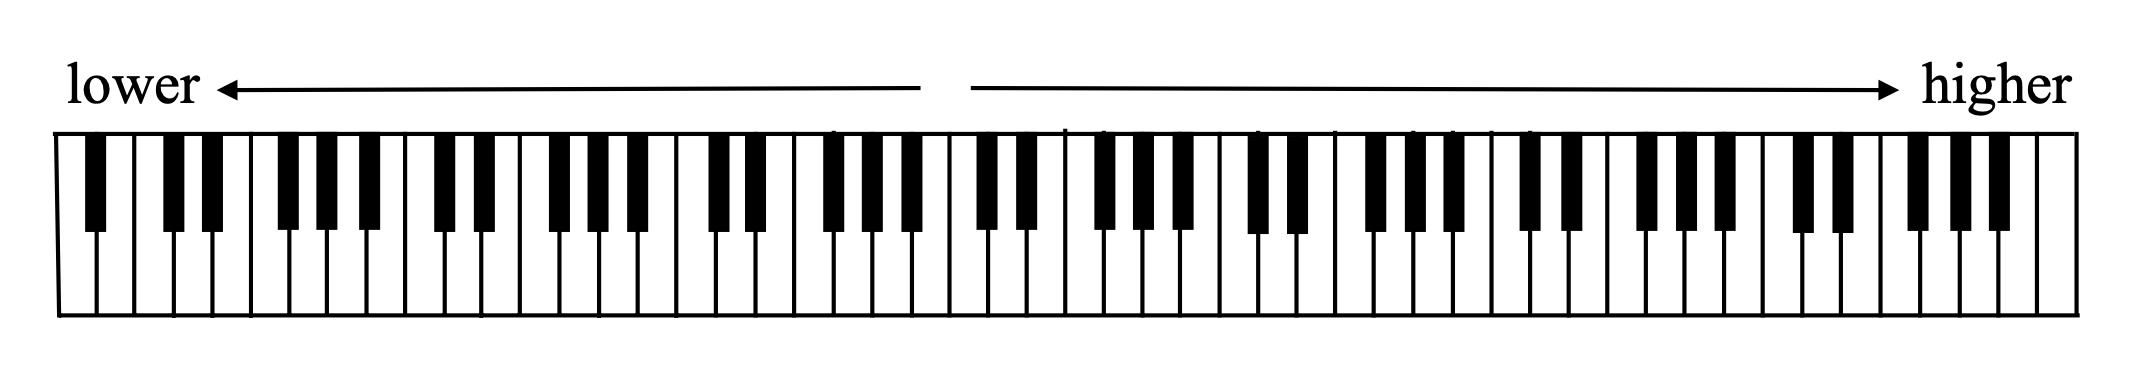
\includegraphics[width=\textwidth]{assets/piano}
    \caption{~A piano with 88 keys and indicated pitches~\cite{music-theory}}\label{fig:piano}
\end{figure}


\section{Notation}\label{sec:notation}

Notes are written on a five-line \textit{staff} (figure~\ref{fig:staff}).
A \textit{clef} orients the lines to a reference point.
For example, when placed on a five-line staff, the \textit{G clef} becomes the \textit{treble clef}, the most well-known \textit{clef}.
In treble clef, the notes on the lines are E--G--B--D--F from lowest to highest, often remembered through the traditional mnemonic\footnote{Every Good Boy Does Fine}.
The spaces are F--A--C--E from lowest to highest.
\textit{Staves} (the plural of ``staff'') are extended by the ledger lines (figure~\ref{fig:staff}).~\cite{music-theory}


\begin{figure}
    \centering
    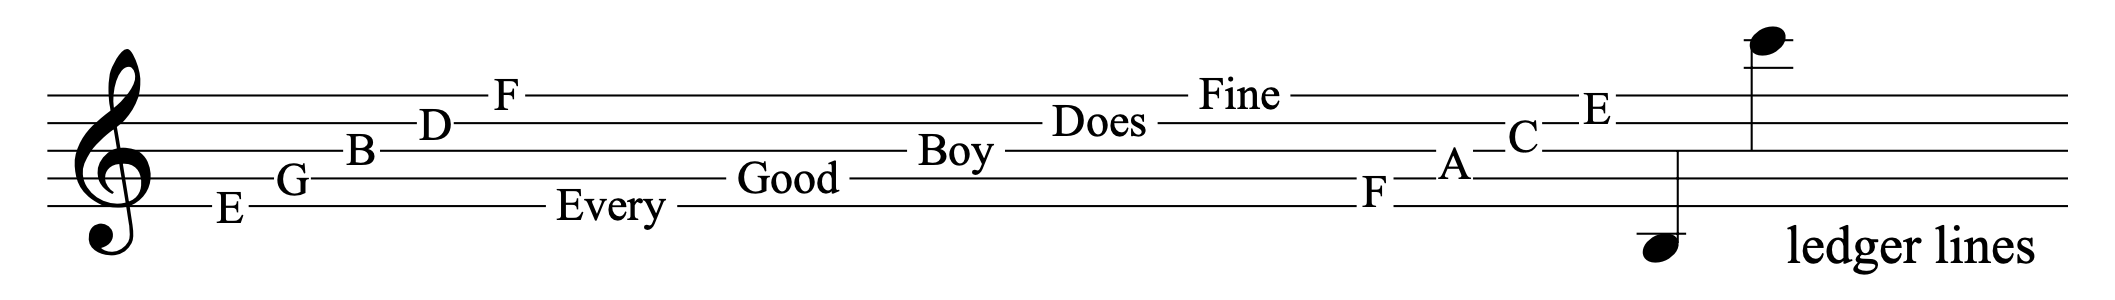
\includegraphics[width=\textwidth]{assets/staff}
    \caption{~The staff with a treble clef~\cite{music-theory}}\label{fig:staff}
\end{figure}


\section{Octave registers}\label{sec:octave-registers}

The note names used in music are \textit{ABCDEFG} (known as the ``musical alphabet'').
After G, note A returns, and \textit{ABCDEFG} occurs again.
An octave is a distance from any note to the same note in the next or previous register.
A piano also contains so-called \textit{accidentals} (special keys that raise or lower a note's pitch).
The piano keyboard with 88 notes consists of seven octaves (composed of seven notes and five accidentals) along with three extra notes and one extra accidental.~\cite{music-theory}

When learning about octave registers, we focus on note C for reasons that will soon become clear after learning about the major scale.
We use octave registers (C4, D5, \ldots) to specify the note's exact register.
The note C4 is known as \textbf{``middle C''} and is a vital reference point.
See the keyboard in the figure~\ref{fig:octave-registers}.~\cite{music-theory}

\begin{figure}
    \centering
    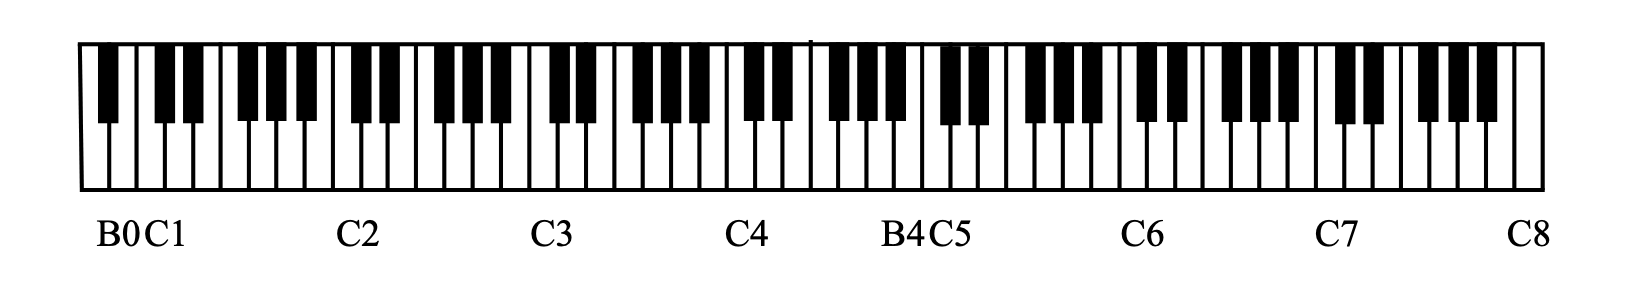
\includegraphics[width=\textwidth]{assets/octave-registers}
    \caption{~A piano with octave registers denoted~\cite{music-theory}}\label{fig:octave-registers}
\end{figure}

Notice that the register number changes after note B each time (e.g., B4 is followed by C5).
In the treble clef notation, middle C is placed on the \textit{ledger line} below the staff.
In the bass clef, the \textit{middle C} is placed on the \textit{ledger line} above the staff.
Both notations are visible in figure~\ref{fig:middle-c}.~\cite{music-theory}

\begin{figure}
    \centering
    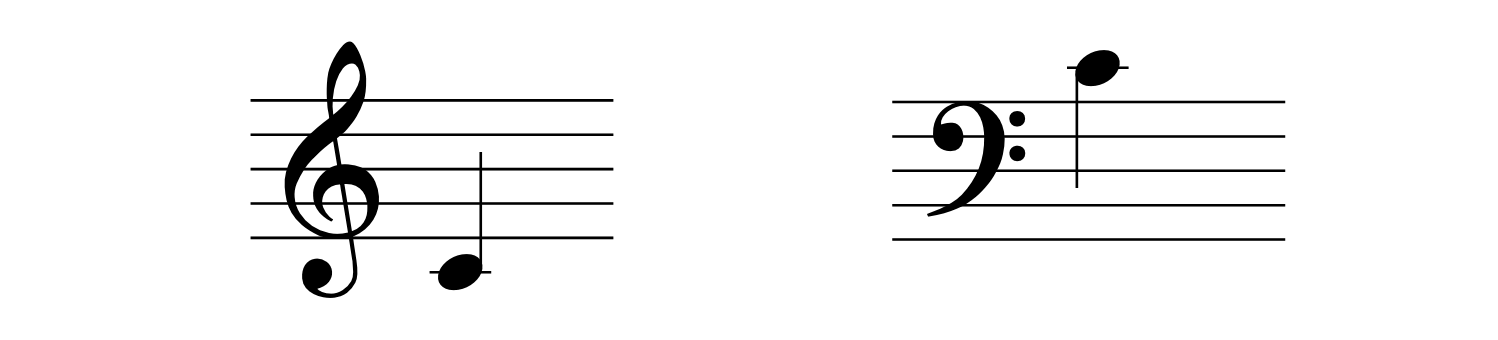
\includegraphics[width=\textwidth]{assets/middle-c}
    \caption{~Middle C (C4) in treble clef and bass clef~\cite{music-theory}}\label{fig:middle-c}
\end{figure}

When we join the treble and the bass clef together by a bracket, we create the so-called \textbf{grand staff}, how piano music is written.
An example of the \textbf{grand staff} is shown in figure~\ref{fig:grand-staff}.~\cite{music-theory}


\begin{figure}
    \centering
    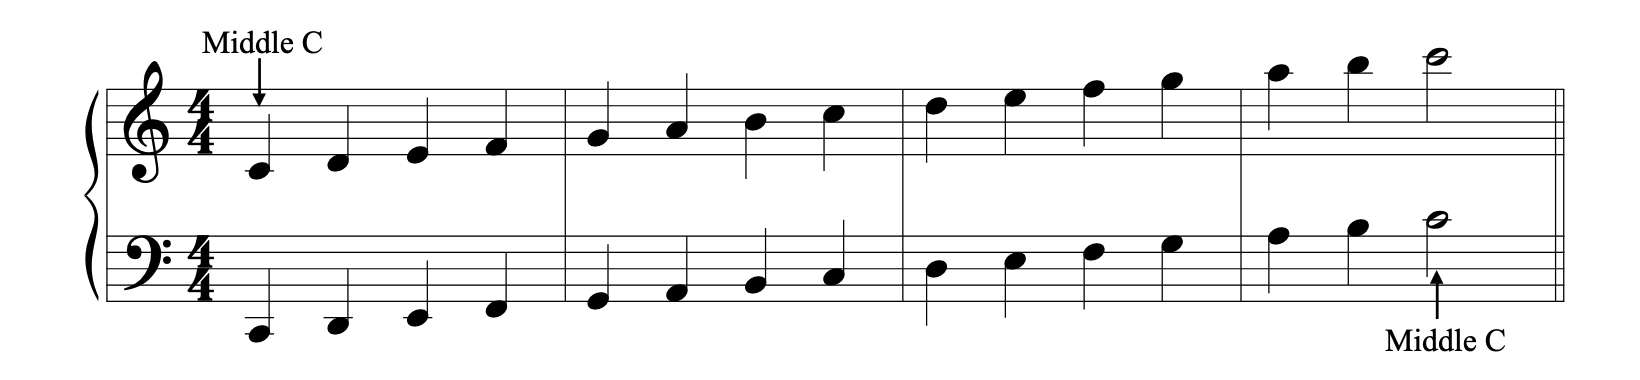
\includegraphics[width=\textwidth]{assets/grand-staff}
    \caption{~The grand staff~\cite{music-theory}}\label{fig:grand-staff}
\end{figure}


\section{Accidentals}\label{sec:accidentals}

Accidentals are characters that we use to modify the following note (either raise or lower the note pitch).
The following five symbols exist~\cite{music-theory}:

\begin{itemize}
    \item \textit{Sharp} symbol (\sh) raises pitch half a step
    \item \textit{Flat} symbol (\fl) lowers pitch half a step
    \item Double \textit{sharp} symbol (\musDoubleSharp) raises pitch two halves a step (a whole step)
    \item Double \textit{flat} symbol (\musDoubleFlat) lowers pitch two halves a step (a whole step)
    \item \textit{Natural} symbol (\na) cancels out accidentals previously applied in a measure of Major Key Signatures or Minor Key Signatures
\end{itemize}


\section{Half Steps and Whole Steps}\label{sec:half-whole-steps}

A half step on a piano keyboard is the distance from one note to the following immediate note.
A whole step composes of two half steps (figure~\ref{fig:half-whole-steps}).~\cite{music-theory}


\begin{figure}
    \centering
    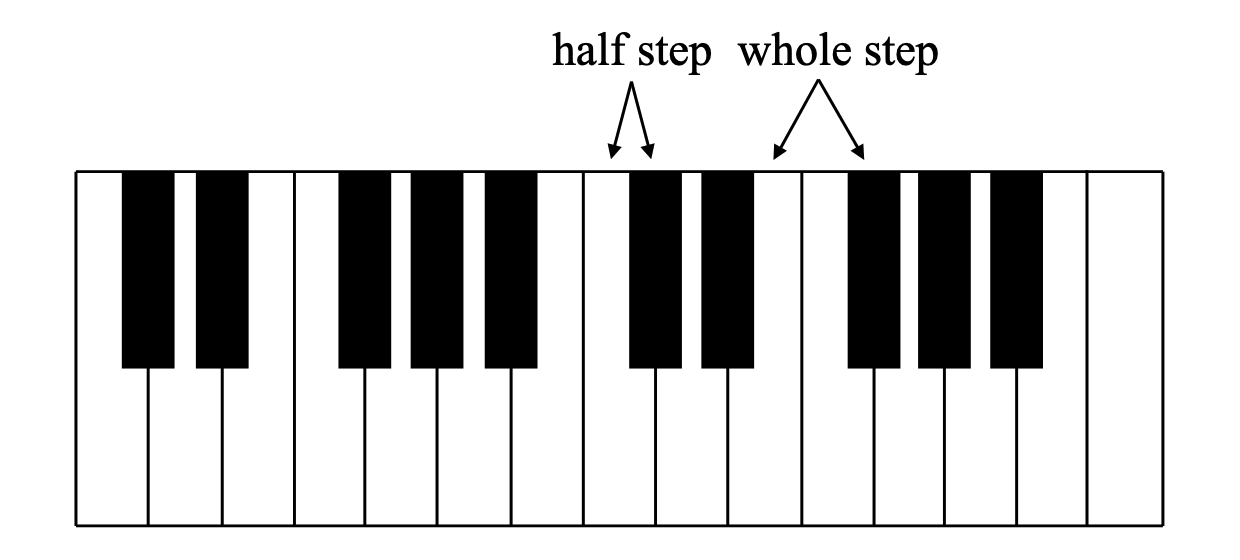
\includegraphics[width=0.78\textwidth]{assets/half-whole-steps}
    \caption{~The half step and whole step~\cite{music-theory}}\label{fig:half-whole-steps}
\end{figure}


\section{The Major scale}\label{sec:major-scale}

A specific sequence of whole and half steps is called a \textit{major scale}.
It is helpful to think of the pattern as consisting of two \textit{tetrachords}\footnote{\textit{``a tetrachord is a four-note scale segment''~\cite{music-theory}}} and a single whole step.
The lower \textit{tetrachord} is of the following pattern: whole step, whole step, half step.
A whole step then joins both \textit{tetrachords} together.
The upper \textit{tetrachord} consists of the same pattern as the lower one: whole step, whole step, half step.
If we use W for the whole step and H for the half step, we can write the major scale pattern as W--W--H, Whole–step connection, W--W--H.~\cite{music-theory}


\begin{figure}
    \centering
    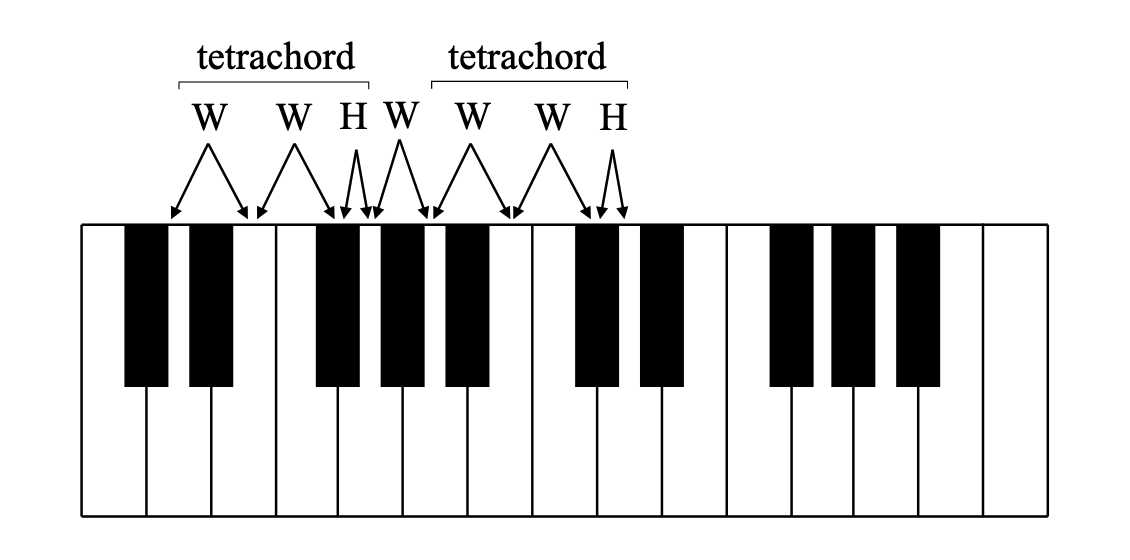
\includegraphics[width=0.8\textwidth]{assets/major-scale-keyboard}
    \caption{~The D major scale on a keyboard~\cite{music-theory}}\label{fig:major-scale-keyboard}
\end{figure}


\begin{figure}
    \centering
    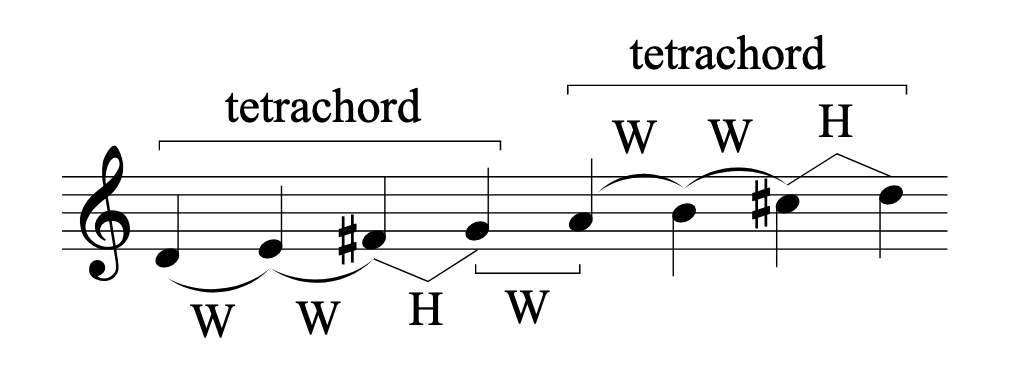
\includegraphics[width=0.84\textwidth]{assets/major-scale-staff}
    \caption{~The D major scale in treble clef~\cite{music-theory}}\label{fig:major-scale-staff}
\end{figure}

Note that all \textit{major scales} use the notes of the musical alphabet in order;
no notes get skipped, and no note occurs twice.
In figure~\ref{fig:major-scale-staff}, the first four notes are D--E--F\textsuperscript{\sh}--G, not D--E--G\textsuperscript{\fl}--G.
In D--E--G\textsuperscript{\fl}--G, G incorrectly occurs twice, and the F\textsuperscript{\sh} between E and G gets skipped.~\cite{music-theory}


\section{Major key signatures}\label{sec:major-key-signatures}

The key signature is a notation positioned next to the clef at the beginning of a piece or section.
We use it to hint which sharps or flats are in the piece's scale to prevent the composer from writing every sharp/flat from the scale each time it occurs.~\cite{music-theory}

There are \textbf{15} major \textit{key signatures}.
The key of \textit{C major has no sharps or flats} in the key signature, while the other key signatures can have between \textit{1 to 7 sharps} and \textit{1 to 7 flats}, resulting in the other 14 key signatures.
Notations of the major key signatures can be seen in figures 23 and 24 for sharps and flats, respectively.~\cite{music-theory}


\begin{figure}
    \centering
    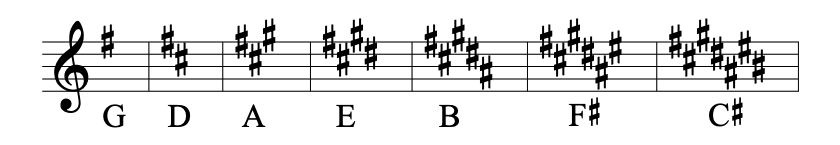
\includegraphics[width=\textwidth]{assets/major-signatures-sharps}
    \caption{~Major key signatures in sharps~\cite{music-theory}}\label{fig:major-signatures-sharps}
\end{figure}


\begin{figure}
    \centering
    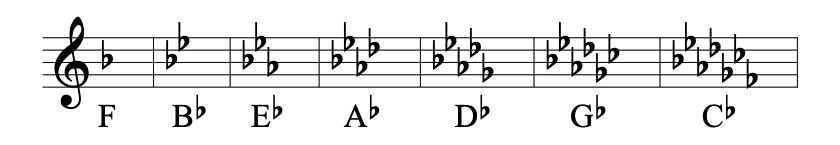
\includegraphics[width=\textwidth]{assets/major-signatures-flats}
    \caption{~Major key signatures in flats~\cite{music-theory}}\label{fig:major-signatures-flats}
\end{figure}

\textit{``A helpful learning device to remember the order of keys in relation to the order of sharps and flats is the \textbf{circle of fifths}.
As you ascend in fifths (clockwise), key signatures get one degree `sharper.'
    (C to G is a fifth because C=1, D=2, E=3, F=4, and G=5.)
    As you descend in fifths (counterclockwise), key signatures get one degree `flatter.'{''}}~\cite{music-theory}~(figure~\ref{fig:circle-of-fifths})


\begin{figure}
    \centering
    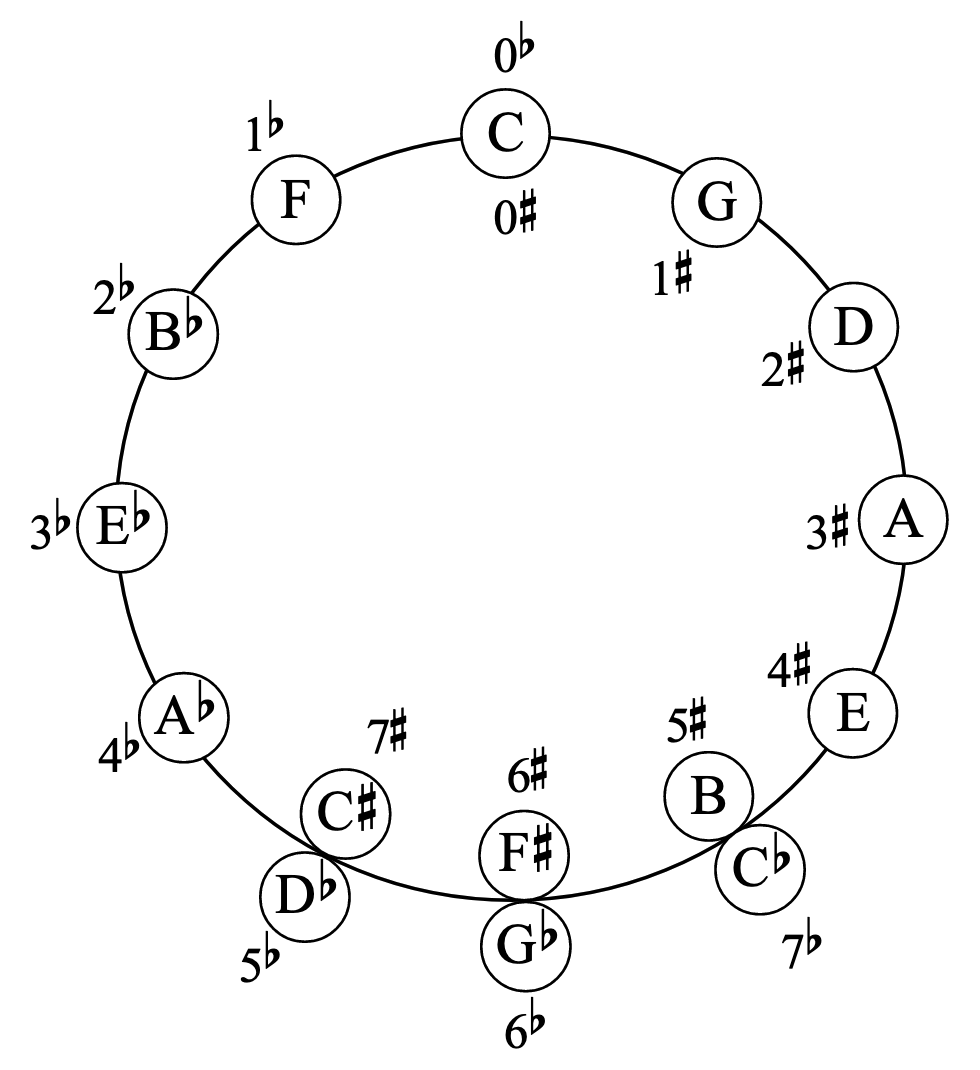
\includegraphics[width=0.6\textwidth]{assets/circle-of-fifths}
    \caption{~Circle of fifths in major keys~\cite{music-theory}}\label{fig:circle-of-fifths}
\end{figure}

Notice the overlapping keys at the bottom of the circle.
B major is enharmonically\footnote{pitches that are the same notes on a piano but are written differently on the staff} the same as C\textsuperscript{\fl} major, F\textsuperscript{\sh} major is enharmonically the same as G\textsuperscript{\fl} major, and C\textsuperscript{\sh} major is enharmonically the same as D\textsuperscript{\fl} major.~\cite{music-theory}


\section{Minor scales}\label{sec:minor-scales}

Alongside the \textit{major scale}, there are also three \textit{minor scales}: the \textit{natural minor scale}, the \textit{harmonic minor scale}, and the \textit{melodic minor scale}.
The \textit{melodic minor scale} has an ascending version, and a descending version that is the same as the \textit{natural minor scale}.
Both can be seen in figure~\ref{fig:minor-scale}.


\begin{figure}
    \centering
    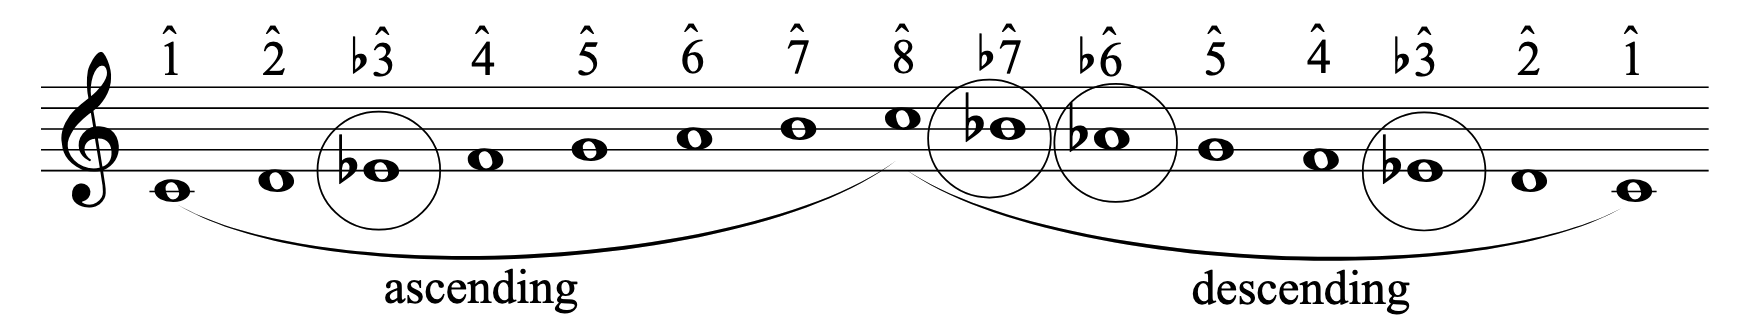
\includegraphics[width=\textwidth]{assets/minor-scale}
    \caption{~Melodic minor scale~\cite{music-theory}}\label{fig:minor-scale}
\end{figure}


\section{Minor key signatures}\label{sec:minor-key-signatures}

\textit{Minor key signatures} agree with the notes of the natural minor scale.
Since the C natural minor scale had E\textsuperscript{\fl}, A\textsuperscript{\fl} and B\textsuperscript{\fl} accidentals, the key signature of C minor has three flats, written in the order of flats (B\textsuperscript{\fl}, E\textsuperscript{\fl}, A\textsuperscript{\fl}).~\cite{music-theory}


\begin{figure}
    \centering
    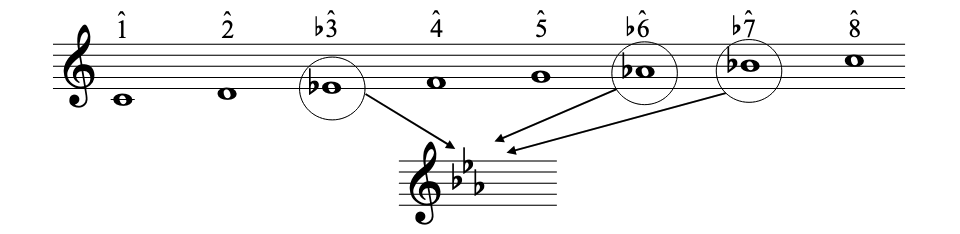
\includegraphics[width=\textwidth]{assets/natural-in-major}
    \caption{~Natural minor scale in major key signature~\cite{music-theory}}\label{fig:natural-in-major}
\end{figure}


\begin{figure}
    \centering
    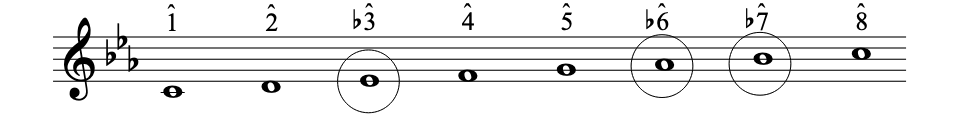
\includegraphics[width=\textwidth]{assets/natural-in-minor}
    \caption{~Natural minor scale in minor key signature~\cite{music-theory}}\label{fig:natural-in-minor}
\end{figure}


A \textit{minor key signature} will have three lowered notes—the third, sixth and seventh—related to the corresponding major key signature.
We use the term \textit{parallel minor} when referring to a minor scale (e.g., the parallel major of F minor is F major) with the same first scale degree (in this case C) as the major.
One method of figuring out a minor key signature is to add three flats (or subtract three sharps) to the parallel major key signature.
When writing below the five-line staff to designate keys, we use upper case for major keys and \textit{lowercase for minor keys}.
~\cite{music-theory}


\begin{figure}
    \centering
    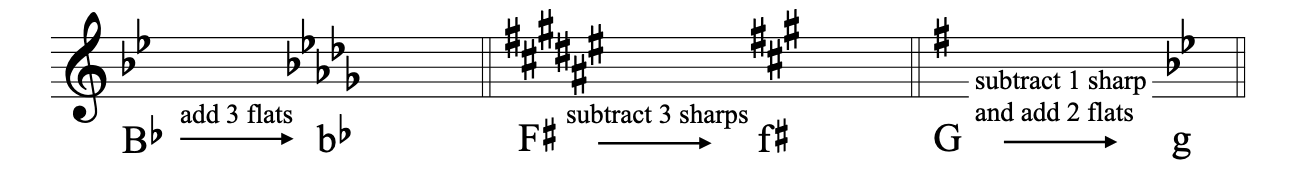
\includegraphics[width=\textwidth]{assets/parallel-minors}
    \caption{~Parallel minor keys signatures~\cite{music-theory}}\label{fig:parallel-minors}
\end{figure}

We also add figures of minor key signatures (figure~\ref{fig:minor-key-signatures}) and circle of fifths (figure~\ref{fig:circle-of-fifths-minor}) for minor scale for completeness.


\begin{figure}
    \centering
    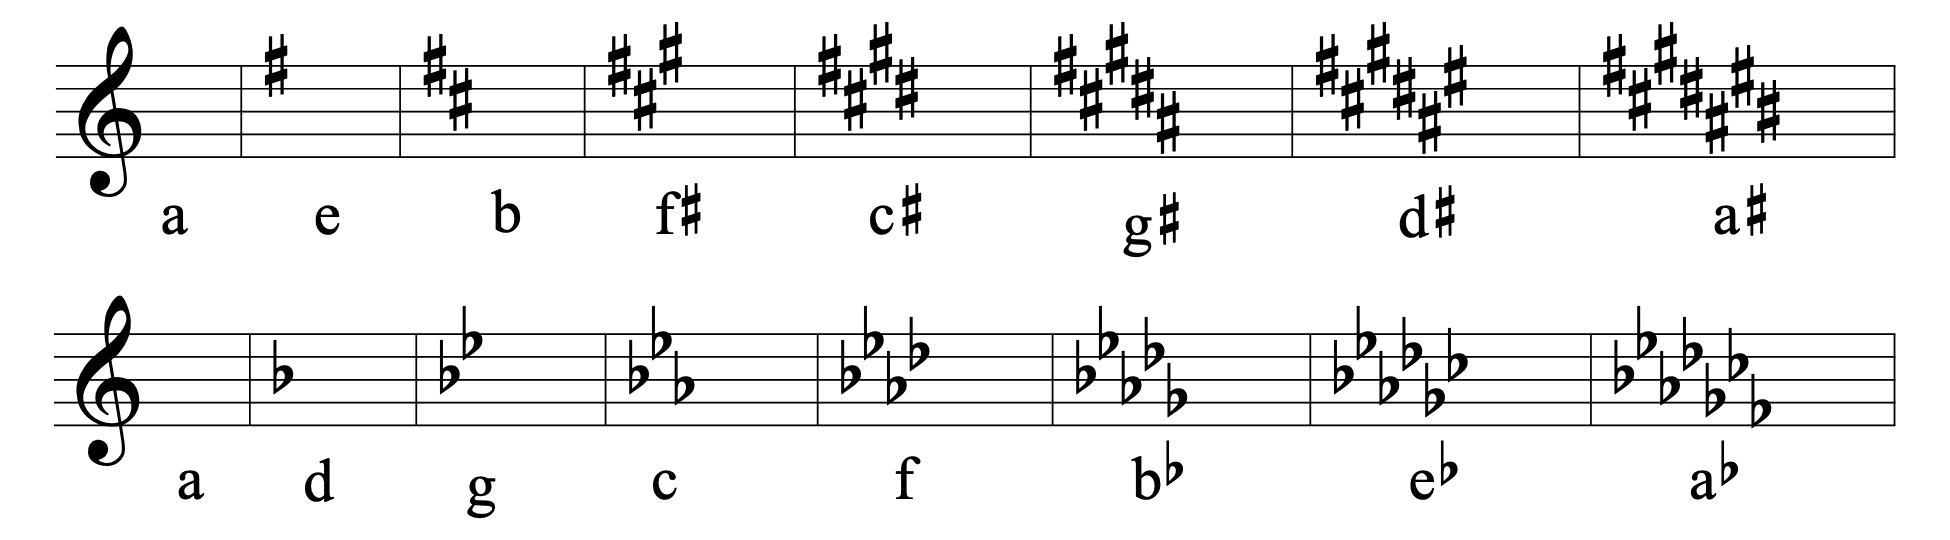
\includegraphics[width=\textwidth]{assets/minor-key-signatures}
    \caption{~Minor keys signatures~\cite{music-theory}}\label{fig:minor-key-signatures}
\end{figure}



\begin{figure}
    \centering
    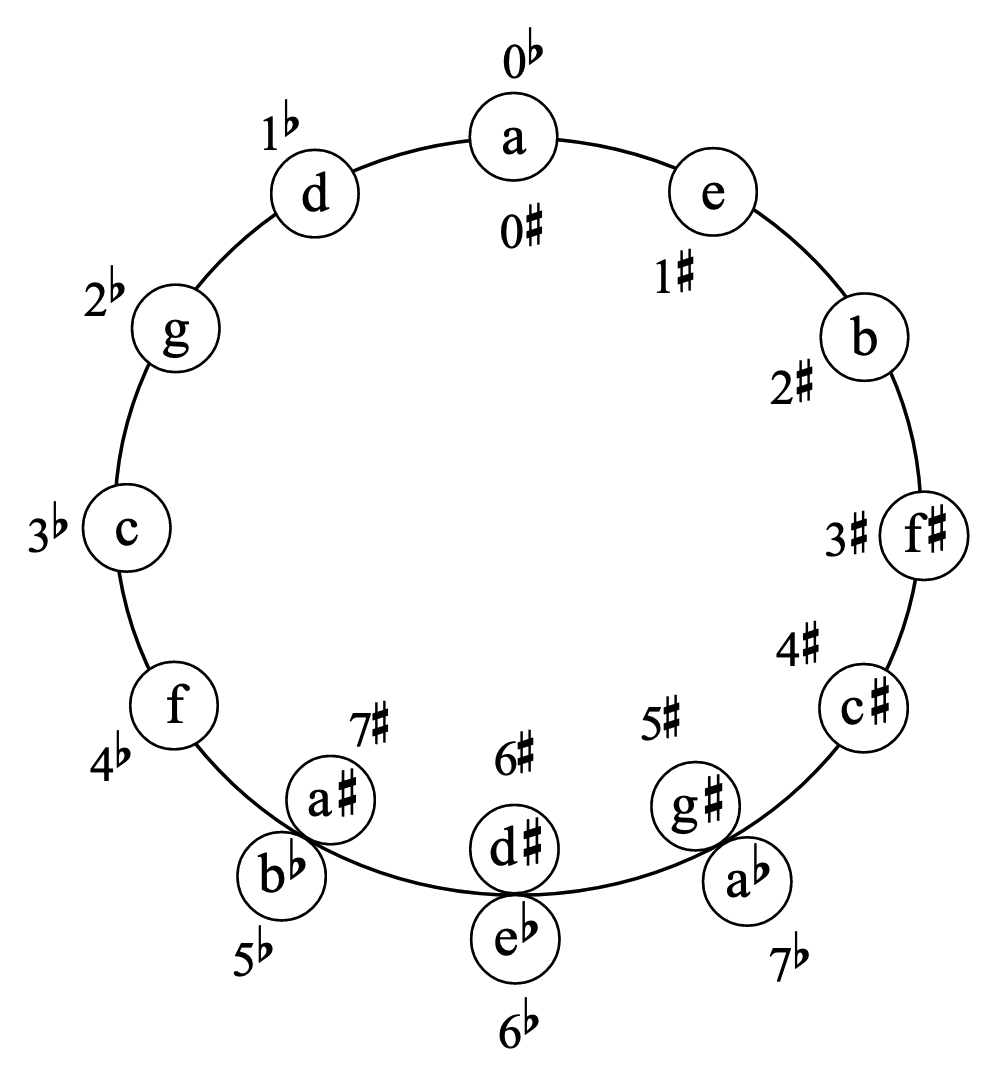
\includegraphics[width=0.6\textwidth]{assets/circle-of-fifths-minor}
    \caption{~Circle of fifths in minor keys~\cite{music-theory}}\label{fig:circle-of-fifths-minor}
\end{figure}


\section{Time signature}\label{sec:time-signature}


The staff can also contain a \textit{time signature} next to a clef.
We denote it as two stacked numbers;
the lower number is typically a number corresponding to a power of 2 and tells us the relative duration of a note, while the upper number hints at how many pulses (or \textit{beats}) we can expect per \textit{bar}\footnote{specified segment of time corresponding to the number of beats}.~\cite{music-theory}


\begin{figure}
    \centering
    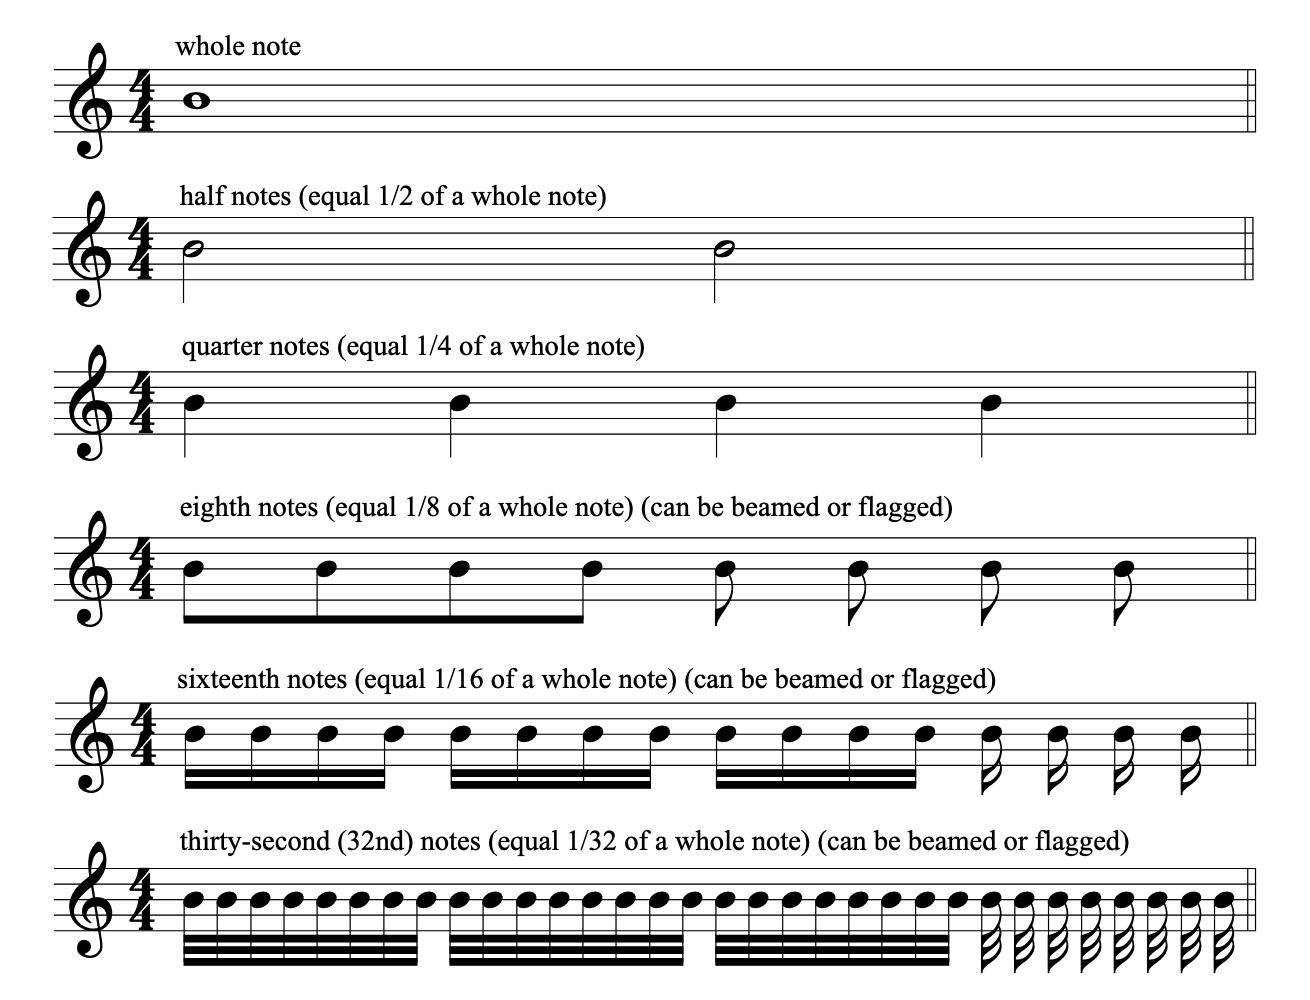
\includegraphics[width=0.8\textwidth]{assets/common-time-notes}
    \caption{~Different notes used for a common time~\cite{music-theory}}\label{fig:common-time-notes}
\end{figure}


\section{Durational symbols}\label{sec:durational-symbols}

The most common \textit{time signature} is $_{4}^{4}$ (also known as ``common time'').
It makes sense to introduce \textit{durational symbols} in the context of $_{4}^{4}$ time signature because a whole note takes up a full measure in $_{4}^{4}$, a half note takes up half a measure of $_{4}^{4}$, a quarter note takes up $\frac{1}{4}$ of a measure, and so on.


\begin{figure}
    \centering
    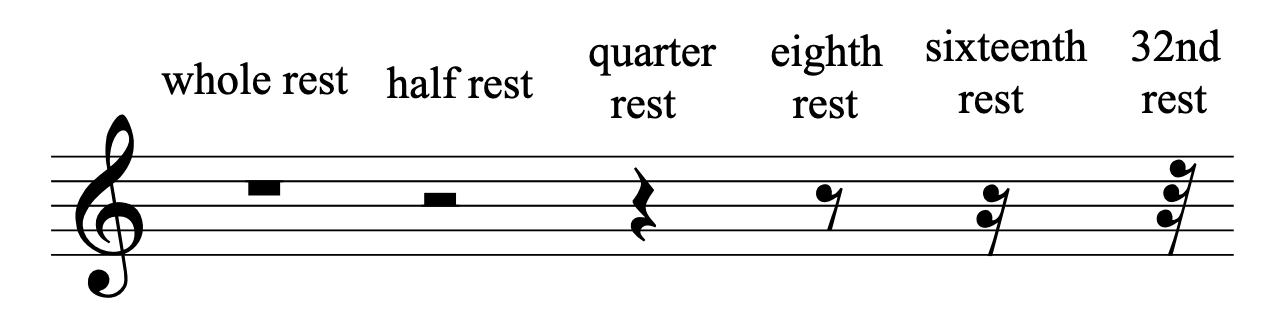
\includegraphics[width=0.9\textwidth]{assets/durational-symbols}
    \caption{~Durational symbols for rests~\cite{music-theory}}\label{fig:durational-symbols}
\end{figure}

Meter describes the number of beats in a measure (also called a bar) and how we typically divide the beats.
A beat is a basic pulse measured in music and thus the unit in which we think about music.
Pulse and beat are interchangeable.
The speed of a beat is called tempo.
We can state tempo in beats per minute (\textit{bpm}), such as 60bpm (where the rate of the beat would be equal to a second), or, in classical music, with terms like Allegro, Andante, and Adagio, sometimes in combinations with ``M.M.'' for Maelzel's Metronome.~\cite{music-theory}

Some meters have a special name;
meters with two beats in a bar are called \textit{duple}, three beats in a bar \textit{triple}, and four beats in a bar \textit{quadruple}.
Meter is described as \textit{simple} if the beats are normally divided into two parts and \textit{compound} if the beats are normally divided into three parts.~\cite{music-theory}



% Automated music generation
%---------------------------------------------------------------


\addcontentsline{toc}{chapter}{Automated music generation}
\markboth{Automated music generation}{Automated music generation}

\begin{chapterabstract}
    When talking about \textit{automated music generation}, we may want to distinguish between \textit{composition assistance} (software that is not generating the music from scratch but instead helps the composer incrementally with suggestions, auto-completion, etc.) and \textit{autonomous music generation} (which takes over the whole music composing process and users are restricted just to parametrization of the generation process).
    In this chapter, we will focus on the latter.
    We will briefly go over the history of the music generation and then move on to modern techniques utilizing machine learning techniques.~\cite{music-generation-history}
\end{chapterabstract}


\section{Pre-computer techniques}\label{sec:pre-computer-techniques}

First experimentations with \textit{algorithmic composition} took place in the late 15th century by employing \textbf{"canonic composition."}~\cite{brief-history-of-algo-composition}

\textit{``The prevailing method was to write out a single voice part and to give instructions to the singers to derive the additional voices from it.
The instruction or rule by which these further parts were derived was called a canon, which means `rule' or `law.' For example, the second voice might be instructed to sing the same melody starting a certain number of beats or measures after the original;
the second voice might be an inversion of the first or it might be a retrograde [etc.]''}~\cite{history-of-western-music}

These \textit{rules} of imitation and manipulation form an \textit{algorithm} by which performers unfold the music.
In this automatical process, we see a clear removal of the composer from a large portion of the compositional process: the composer himself only invents a core of the music, a single melody or section.~\cite{brief-history-of-algo-composition}

\textit{Wolfgang Amadeus Mozart} experimented with automated composition techniques using the so-called \textit{Musikalisches Wurfelspiel} (``musical dice game'').
The game worked by joining several predefined musical segments selected by dice roll.
This simple form of \textit{stochastic} algorithmic composition left the creative decisions in the hands of chance, letting the dice roll decide what notes to use.~\cite{brief-history-of-algo-composition}


\section{Use of computers}\label{sec:use-of-computer}

There are three possible approaches when using a computer to generate a composition:
\begin{itemize}
    \item Stochastic
    \item Rule-based
    \item Artificial intelligence
    % TODO: describe the items
\end{itemize}

The \textit{stochastic} way involves \textit{randomness} and can be as simple as Mozart's \textit{Musical dice game} we already briefly touched upon;
however, we can also use more complex methods like \textit{statistical theory} and \textit{Markov chains}.
Many creative decisions are merely left to chance when generating a composition using the stochastic method.
Another example of non-computer-oriented stochastic composition can be found in Karlheinz \textit{Stockhausen's Klaveirstucke XI}, in which the sequence of various fragments of music is to be performed by a pianist in random order.~\cite{brief-history-of-algo-composition}

\subsection{Markov chains}\label{subsec:markov-chains}

So-called \textit{Markov chains} are a major technique for generating musical compositions using stochastics.
We define the Markov chain using a simple sequence of random variables $X_1, X_2, X_3, \ldots, X_i$\footnote{the index $i$ in this context is sometimes referred to as the time}; we call this sequence a \textit{stochastic process}.
For this process to be the Markov chain, the following equivalence must be true:
\[ [X_i\rvert X_1, \ldots, X_{i-1}] \sim [X_i\rvert X_{i-1}] \]
In this context, the equivalence means that the \textit{probability distribution} on the left-hand side is equivalent to the probability distribution on the right-hand side.
For a fixed value of $i$, $X_i$ is called the state of the Markov chain.
The equivalence implies that the value of $i\textsuperscript{th}$ state is purely dependent on the immediately previous state, a trait also called \textit{memoryless}.~\cite{markov-chains}

Markov chains are primarily represented in two ways a \textit{transition matrix} (figure~\ref{fig:markov-chain-matrix}) or a \textit{directed graph} (figure~\ref{fig:markov-chain-graph}).
The transition matrix $M$ is a matrix with dimensions $n$ by $n$, where $n$ is the number of different states the Markov chain maintains.
The $M_{a,b}$ value then represents $\mathcal{P}(b \rvert a)$, the probability of transition from the state $a$ to state $b$.
This representation is practical for use in computers.
The directed graph is a good representation for visualization;
each \textit{vertex} represents a state, and the \textit{directed edges} represent the probability of a transition between two states.~\cite{markov-chains}

\begin{figure}
    \centering
    \[
        \begin{blockarray}{cccc}
            & \text{Sunny}     & \text{Windy}     & \text{Rainy} \\
            \begin{block}{c(ccc)}
                \text{Sunny}     & 0.6     & 0.3     & 0.1 \\
                \text{Windy}     & 0.7     & 0       & 0.3 \\
                \text{Rainy}     & 0.5     & 0.2     & 0.3 \\
            \end{block}%
        \end{blockarray}%
    \]
    \caption{~Markov chain represented by transition matrix~\cite{markov-chains}}\label{fig:markov-chain-matrix}
\end{figure}

\begin{figure}
    \centering
    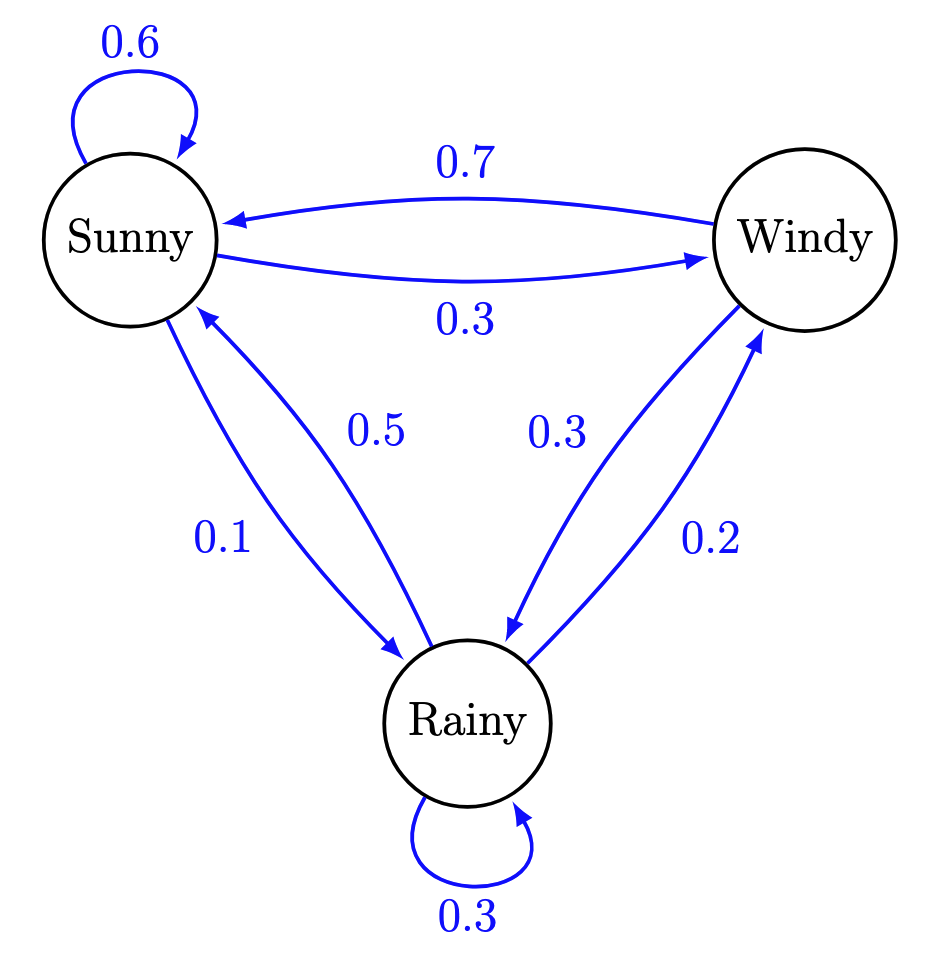
\includegraphics[width=0.5\textwidth]{assets/markov-chain-graph}
    \caption{~Markov chain represented by directed graph~\cite{markov-chains}}\label{fig:markov-chain-graph}
\end{figure}

\subsubsection{Generating music}\label{subsubsec:generating-music}

Once we have the Markov chain defined, we can use it to generate music in a simple manner;
we want to create a model that will contain sound objects (notes or chords and their duration) as states and probabilities of transitions between them.
We do this by using existing music pieces and using them as training input.
We compose the states by extracting all different sound objects occurring in the training pieces.
We can compute the transition probabilities by gathering all possible \textit{bigrams} (sequences of two adjacent objects).
The probability of transition from the state $a$ to state $b$ is then computed by following division $\mathcal{P}(b \rvert a) = \frac{\# ab}{\# ac}$, where $ab$ represents bigrams of sound object $a$ followed by sound object $b$, and $ax$ represents \textit{all bigrams} starting with the object $a$.
Using this method we compose the whole transition matrix.

With the transition matrix available, we can move on to the music generation itself.
In order to utilize the matrix for generating transitions, we first need to select the first sound object the musical piece will start with.
We can do that by manually picking the desired sound object, or we can generate it randomly by composing a vector of probabilities of starting sound objects, where the probability of each object being the starting object is the number of times it was starting object in training musical pieces divided by the total number of training musical pieces.
So to generate the piece, we select starting object from the initial vector (the likelihood of selecting an object is determined by its computed probability).
Then for every other state, we receive the vector of probabilities by using a row of the transition matrix corresponding to the current state.
We iteratively continue until we are satisfied with the length of a piece.~\cite{markov-chains}

\subsection{Rule-based music generation}\label{subsec:rule-based}

Music theory traditionally describes rules that help to direct the compositional process.
While composers regularly break those rules, they can be successfully used to implement a system for generating music.
One of the examples would be the \textit{Illiac Suite}, composed in 1957 by professors \textit{Lejaren Hiller} and \textit{Leonard Issacson}, where the rule-based system was used to help generate the first two movements.~\cite{computational-creativity}

\textit{``The general idea is to use screening rules to accept or reject randomly generated pitches and rhythms.
Probability distribution and Markov processes can also be found in the suite.''}~\cite{illiac-suite}

\subsubsection{Formal Grammars}\label{subsubsec:formal-grammars}

In the 1950s, \textit{Noam Chomsky} introduced the concept of \textit{Generative Grammars}, a tool for analyzing language that became highly influential in linguistic studies.
In a Generative Grammar, two alphabets of \textit{terminal} and \textit{non-terminal symbols} are used, along with a set of \textit{rewriting rules} given over the union of these two alphabets that allow transforming non-terminal symbols (or string of non-terminal and terminal symbols) into other symbols (both terminals and non-terminals).
The generated \textit{language} is the set of all possible strings of terminal symbols generated from a special starting variable (usually called $S$) and applying any number of rewriting rules in sequence.
These Grammars can be seen as an implementation of the beforementioned rule-based systems.~\cite{computational-creativity}

\textit{Lindenmayer Systems} (L-Systems) are a variant of Generative Grammars used for music generation;
the difference from Chomsky's Grammars is that they implement \textit{parallel rewriting}, applying all the rewriting rules at once instead of only one at a time.
This characteristic makes these systems less inclined to generate sequential data, like simple melodies, and have been used to generate stunning visual effects.
When applied to music generation, a common approach was to map visual data generated by \textit{L-systems} to score information or to a sequence of musical segments.~\cite{computational-creativity}

One of the most influential researchers of rule-based music generation is \textit{Ebcioǧlu}, who implemented a custom logic language that he used to create \textsl{CHORAL}, a system for the generation of Bach-like chorales that uses some 350 rules for harmonization and generation of melodies~\cite{ebcioglu}.
The hardship of designing such a system lies in the complexity of explicitly coding enough rules, many of which often do not have a formal definition in musicology literature.~\cite{computational-creativity}


\subsection{Artificial intelligence}\label{subsec:artificial-intelligence-music-generation}

\textit{``Artificial Intelligence (AI) is the property of machines, computer programs and systems to perform the intellectual and creative functions of a person, independently find ways to solve problems, be able to draw conclusions and make decisions.''}~\cite{about-ai}

AI is a buzzword that contains two main branches, the original \textit{symbolic AI} and \textit{machine learning}.
The symbolic AI are systems where we capture knowledge using formal mathematical logic, genetic algorithms, state-space search, automated planning,~\ldots~.
The machine learning AI builds models with a set of hidden internal parameters we are trying to fine-tune so that the model performs well on predefined metrics;
this optimization process is called learning.
In this thesis, we will specifically focus on \textit{artificial neural networks}, which are subset of ML techniques.

The increased computational power of computers and the widespread general-purpose GPU programming recently made \textit{deep learning}\footnote{use of ANNs with more than three hidden layers} techniques extremely popular, with applications spanning from \textit{NLP} to \textit{image processing} to \textit{music generation}.

While the interest in these algorithms grew exponentially in the last decade, the first music generation system to use ANNs was that of Peter M. Todd\cite{first-ann-mgs}, who used a three-layered \textit{Recurrent Neural Network} (RNN) to generate monophonic melodies.
Recurrent Networks reuse the results of the computations from previous steps every time a new input is fed, allowing them to encode temporal sequences.
Still, standard feed-forward networks are also an option for music generation.
There is also room for standard feed-forward networks: in 1991, J. P. Lewis trained a network\cite{feed-forward-ann-mgs} with musical patterns ranging from random to well-constructed to learn a measure of ``musicality'' used by his music generation system to select pleasing compositions.

As mentioned, RNNs are a popular choice for music generation.
In particular, \textit{LSTMs}\cite{LSTMs} are a special variant of recurrent networks that use gates to decide the amount of information taken from novel input and what is maintained from older inputs, hence the memory.
The first LSTM used for music generation was applied to blues improvisation\cite{LSTM-mgs}.
Another deep learning approach is that of Generative Adversarial Networks (GANs)\cite{gans};
the concept behind this method is to train two networks at the same time, one generates musical compositions imitating what is learned from real-world examples, and the other tries to discriminate between original and imitated compositions.
As one network gets better, the other must improve as well in order to ``beat'' the other network (therefore making them ``Adversarial'').



% Digital audio representation
%---------------------------------------------------------------


\chapter{Digital representation of music}\label{ch:digital-audio-representation}

\begin{chapterabstract}
    In reality, sounds manifest as continuous \textit{waves} propagating through a medium (like air).
    On the other hand, personal computers are \textit{digital} by design and cannot \textit{easily} represent \textit{continuous} information;
    therefore, when storing audio in a computer, we have to perform conversions for the computer to accommodate our audio track.
    This chapter will look over possible representations of music representation in a computer.
\end{chapterabstract}


\section{Wave representation}\label{sec:wave-representation}

The first possible option when representing an audio track in a computer is to try and capture characteristics of the beforementioned \textit{sound wave}.
In order to manipulate this \textit{continuous signal} via a digital computer, the signal must be digitalized with an \textit{analog-to-digital converter} (A/D).
The converter repeatedly samples the instantaneous \textit{voltage amplitude} of the \textit{analog} input signal at a given sample rate, commonly thousands or tens of thousands of times per second.
In the audio signal, the measured voltage of the input signal is proportional to the sound pressure measured by a device such as a \textit{microphone}.
The final discrete representation of the converted signal created by the converter consists of a sequence of numeric values (hence the term digital) representing the amplitude of the original waveform at evenly spaced points in time.~\cite{sound-representation}

\begin{figure}
    \centering
    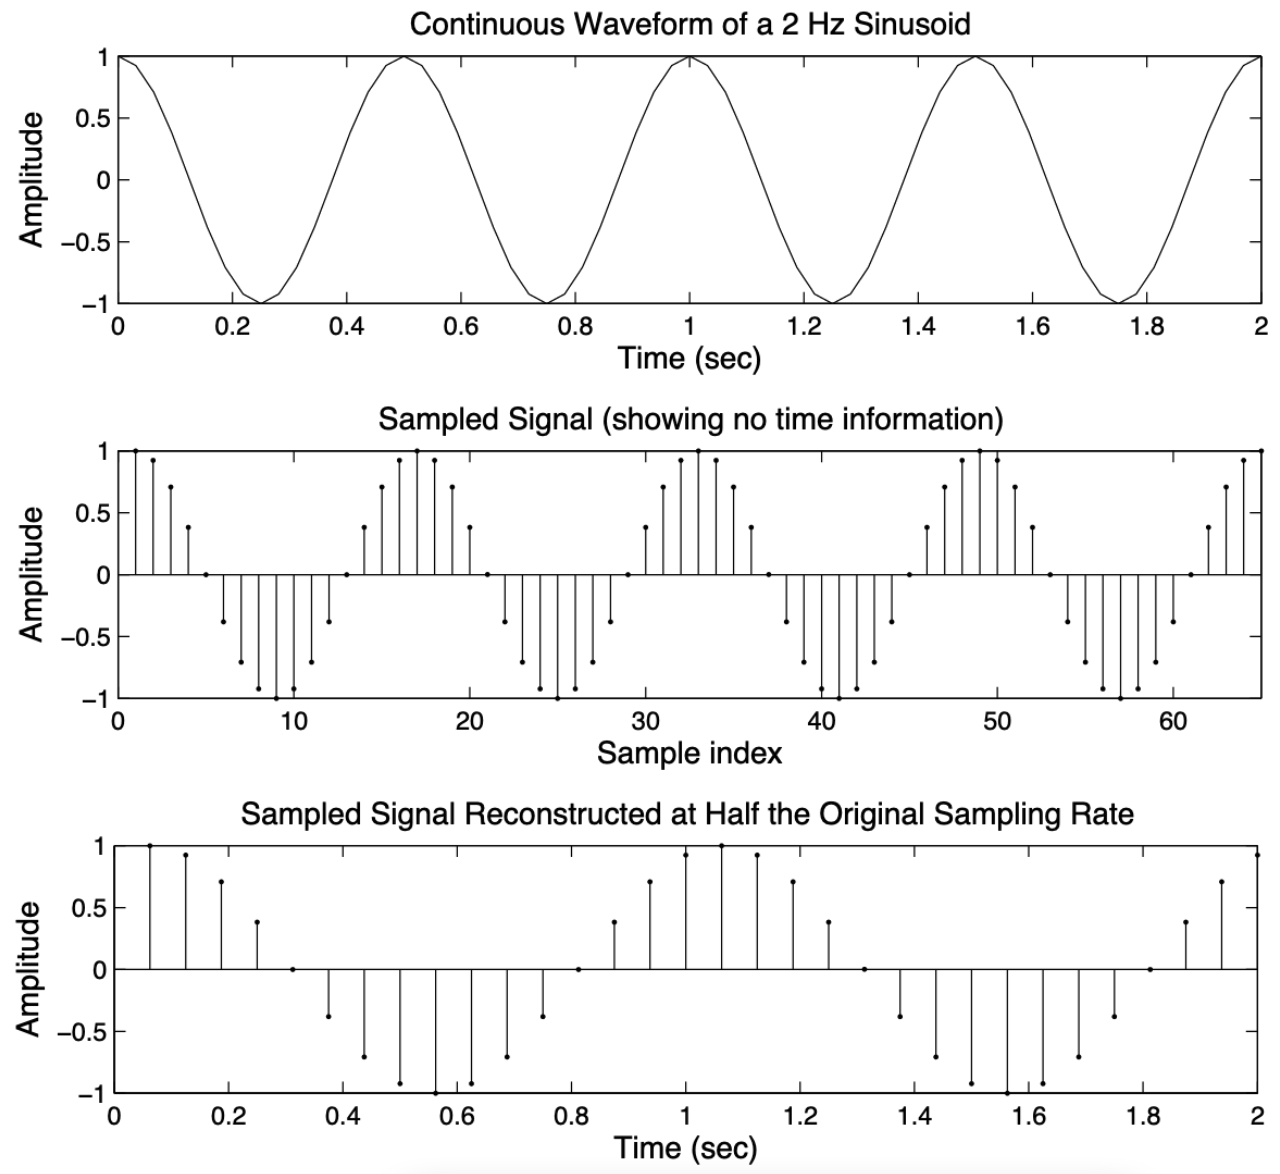
\includegraphics[width=0.7\textwidth]{assets/sound-sampling}
    \caption{~Digitization of signal via sampling~\cite{smyth_2019}}\label{fig:sound-digitization}
\end{figure}


\section{Symbolic representation}\label{sec:symbolic-representation}

Another option is to represent music \textit{symbolically}.
Unlike the wave representation, which represents music (any audio generally) in a low-level physical fashion, the symbolic representation uses \textit{special symbols} to represent different musical elements like notes and rests.

The downside of this representation is that it can only depict specific musical instruments, unlike wave representation, which can also depict vocals and arbitrary sounds.
However, this approach is much better suited for our application, as it expresses the essential musical properties.
Therefore, it will be much easier for our neural nets to learn the intrinsic properties of compositions provided as learning data and thus will presumably be more successful at imitating them.
We will now go over the most common symbolic formats for music.

\subsection{MIDI}\label{subsec:midi}

The MIDI abbreviation stands for the \textit{Musical Instrument Digital Interface}.
It is a protocol developed in the early 1980s to standardize the \textit{exchange and storage} of musical information.
It is the most widespread \textit{binary} communication protocol intended to connect electronic musical instruments such as synthesizers and other electronic music equipment to a computer for recording, editing, and programming.
MIDI protocol appeared as a response to the need to standardize the communication between the synthesizers and other musical equipment and was created when electronic music was developed by a consortium of Japanese and American manufacturers of Synthesizers (Sequential Systems, Roland Corporation, Yamaha, Kurzweil, \ldots).
It is used to transmit data using serial ports but can also be written to a file and be used as a means of storage.
MIDI is an extensive standard consisting of hardware, drivers, communication channels, messages, modes, controllers, visual effects control, and a file format standard.
In this work, we will only concern ourselves with the \textit{MIDI file format}, as it is the thing that we will need during the implementation part.
Since the protocol was developed in the 80s, it was designed to have low overhead and, therefore, \textit{low-level}.
We do not need to go into the detail of binary encoding used to describe different MIDI events;
instead, we will present an abstracted high-level overview, which is sufficient for our application.~\cite{understanding-midi}

\subsubsection{MIDI file format}\label{subsubsec:midi-file-format}

The MIDI file starts with a header, where the format type (single track, multiple synchronous tracks, or multiple asynchronous tracks), the number of tracks, and time division (ticks per beat).
The file body composes of an array of MIDI \textit{messages}.
Each message denotes the message content and $\Delta$ (delta) time;
the amount of ticks the event is shifted after the preceding event.
There are some \textit{meta-messages} that specify additional information like song lyrics, tempo, state end of the track, and others.
There are multiple message types like \texttt{control\_change} for specifying pedal/slider position or program change to choose one of 128 instruments.
However, the most substantial messages are \texttt{note\_on} and \texttt{note\_off}.
These take arguments pitch (0-127) and velocity (0-127) and specify the pressing and releasing of a note specified by pitch number.
The velocity controls the force of a note being pressed.
Zero velocity has the same meaning as the \texttt{note\_off} message, so the release of a key.
Please take a look at figure~\ref{fig:score-to-midi}, which contains an example of a score.~\cite{understanding-midi}

\begin{figure}
    \centering
    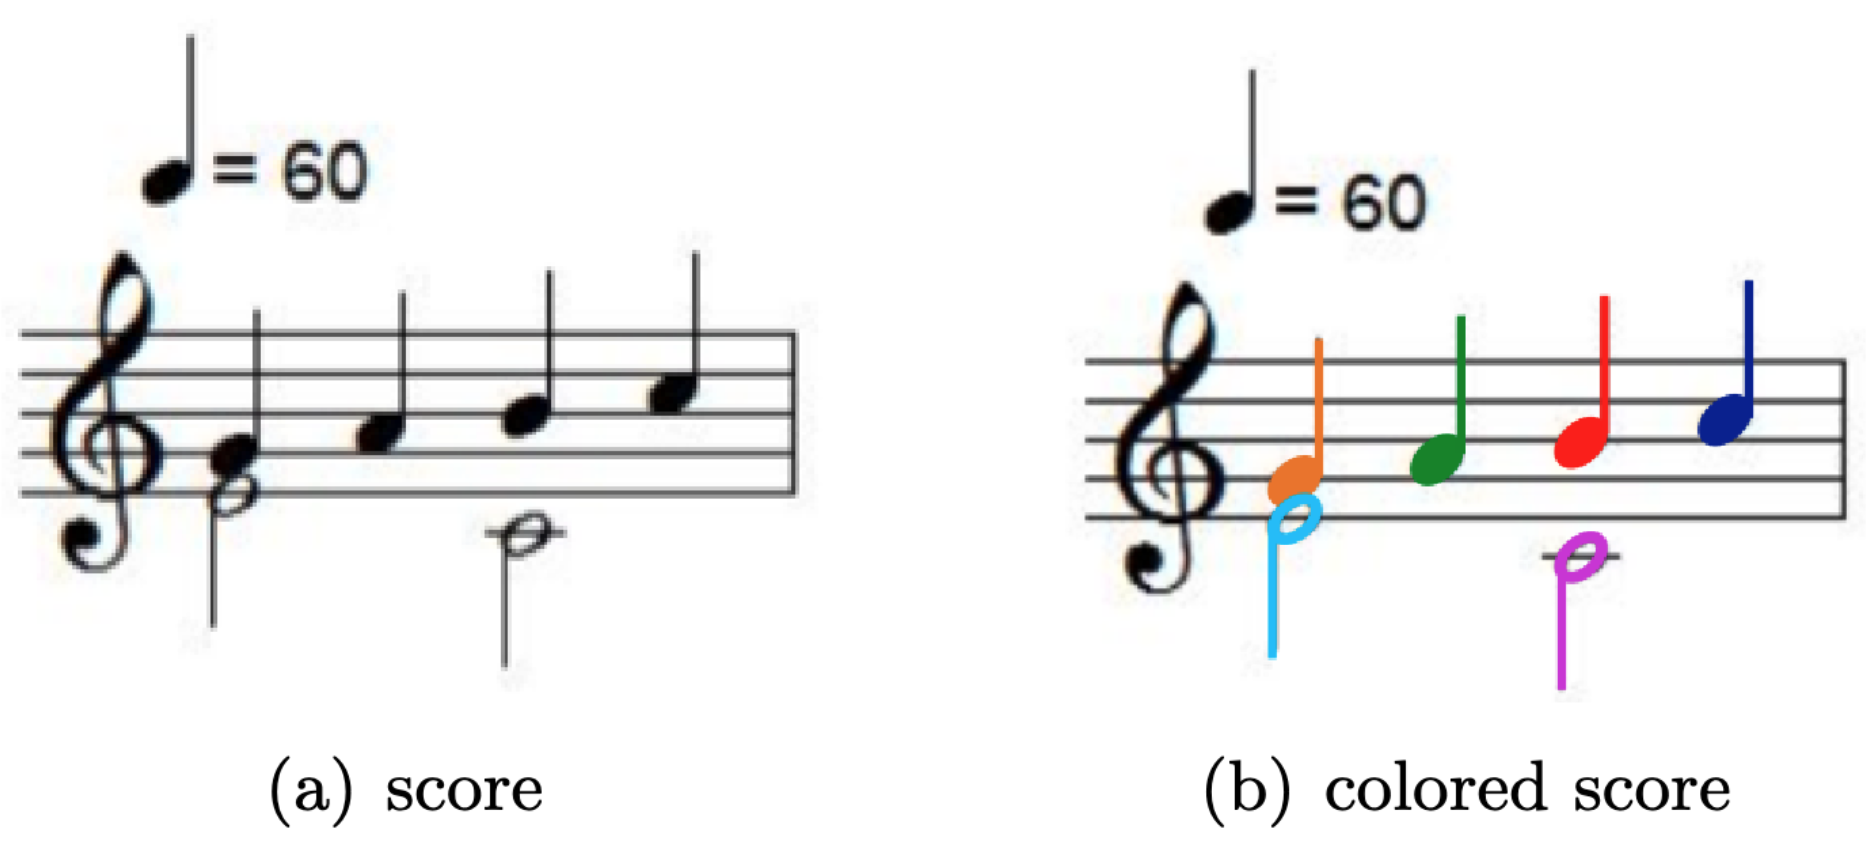
\includegraphics[width=0.4\textwidth]{assets/score-to-midi}
    \caption{~Example of a musical score~\cite{understanding-midi}}\label{fig:score-to-midi}
\end{figure}

This would translate into following messages in MIDI:

\begin{center}
    \begin{tabular}{ |c|c|c| }
        \hline
        \textbf{midi message} & \textbf{pitch} & \textbf{note value}    \\
        \hline
        \texttt{note\_on}     & 64             & \textcolor{cyan}{E4}   \\
        \texttt{note\_on}     & 67             & \textcolor{orange}{G4} \\
        \texttt{note\_off}    & 67             & \textcolor{orange}{G4} \\
        \texttt{note\_on}     & 69             & \textcolor{Green}{A4}  \\
        \texttt{note\_off}    & 69             & \textcolor{Green}{A4}  \\
        \texttt{note\_off}    & 64             & \textcolor{cyan}{E4}   \\
        \texttt{note\_on}     & 60             & \textcolor{violet}{C4} \\
        \texttt{note\_on}     & 71             & \textcolor{red}{B4}    \\
        \texttt{note\_off}    & 71             & \textcolor{red}{B4}    \\
        \texttt{note\_on}     & 72             & \textcolor{blue}{C5}   \\
        \texttt{note\_off}    & 72             & \textcolor{blue}{C5}   \\
        \texttt{note\_off}    & 60             & \textcolor{violet}{C4} \\
        \hline
    \end{tabular}
\end{center}


% Neural networks
%---------------------------------------------------------------


\chapter{Neural networks}\label{ch:neural-networks}


\textit{Artificial neural networks} (ANNs), or just neural networks, are a class of mathematical models used for various tasks, including data classification, self-driving, chatbots, sentiment analysis, time series prediction, computer vision, art generation, and many more.
As the name suggests, ANNs are a set of artificial \textit{neurons} specially arranged into so-called layers.
Neural networks are somewhat inspired by biological neural nets;
hence we will now briefly examine them.~\cite{ann-basics}

The brain consists of many neurons (figure~\ref{fig:bio-neuron}) consisting of dendrites, a cell body, and an axon.
Dendrites are branched connections of a neuron that received propagate the electrochemical stimulation received from other neurons and send them to the cell body, where the signals are summed up, and once the triggering threshold is reached, the signal propagates through the axon.
The last part of a neuron is the axon, the long connection leading from a neuron that transmits a signal to different neurons, muscles, or glands.
Neurons can communicate with other neurons' dendrites and other body parts via these connections, so-called synapses, and pass on their electrochemical potential.
A depiction of the triggering threshold and voltage output is illustrated in figure~\ref{fig:bio-neuron-activation}.~\cite{ann-basics}

\begin{figure}
    \centering
    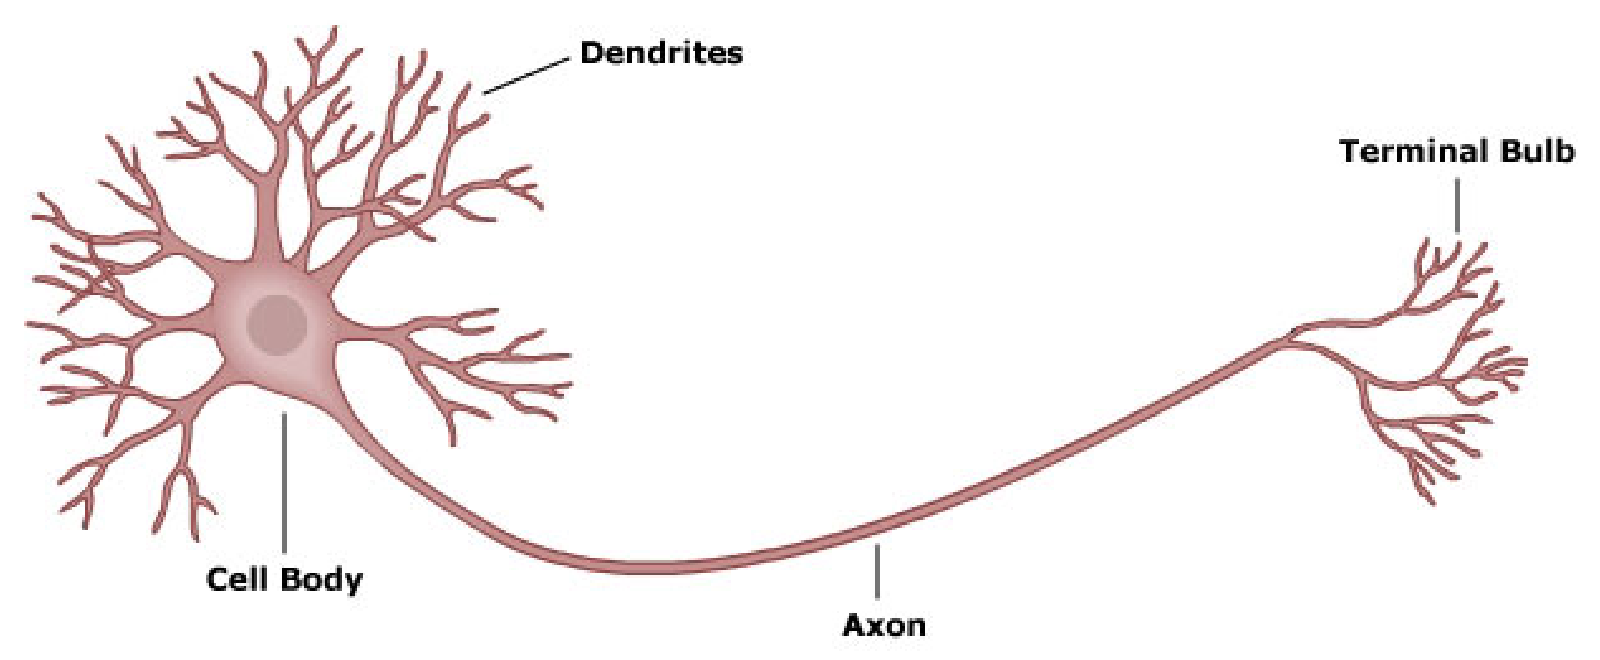
\includegraphics[width=0.74\textwidth]{assets/biological-neuron}
    \caption{~A typical biological neuron~\cite{ann-basics}}\label{fig:bio-neuron}
\end{figure}


\begin{figure}
    \centering
    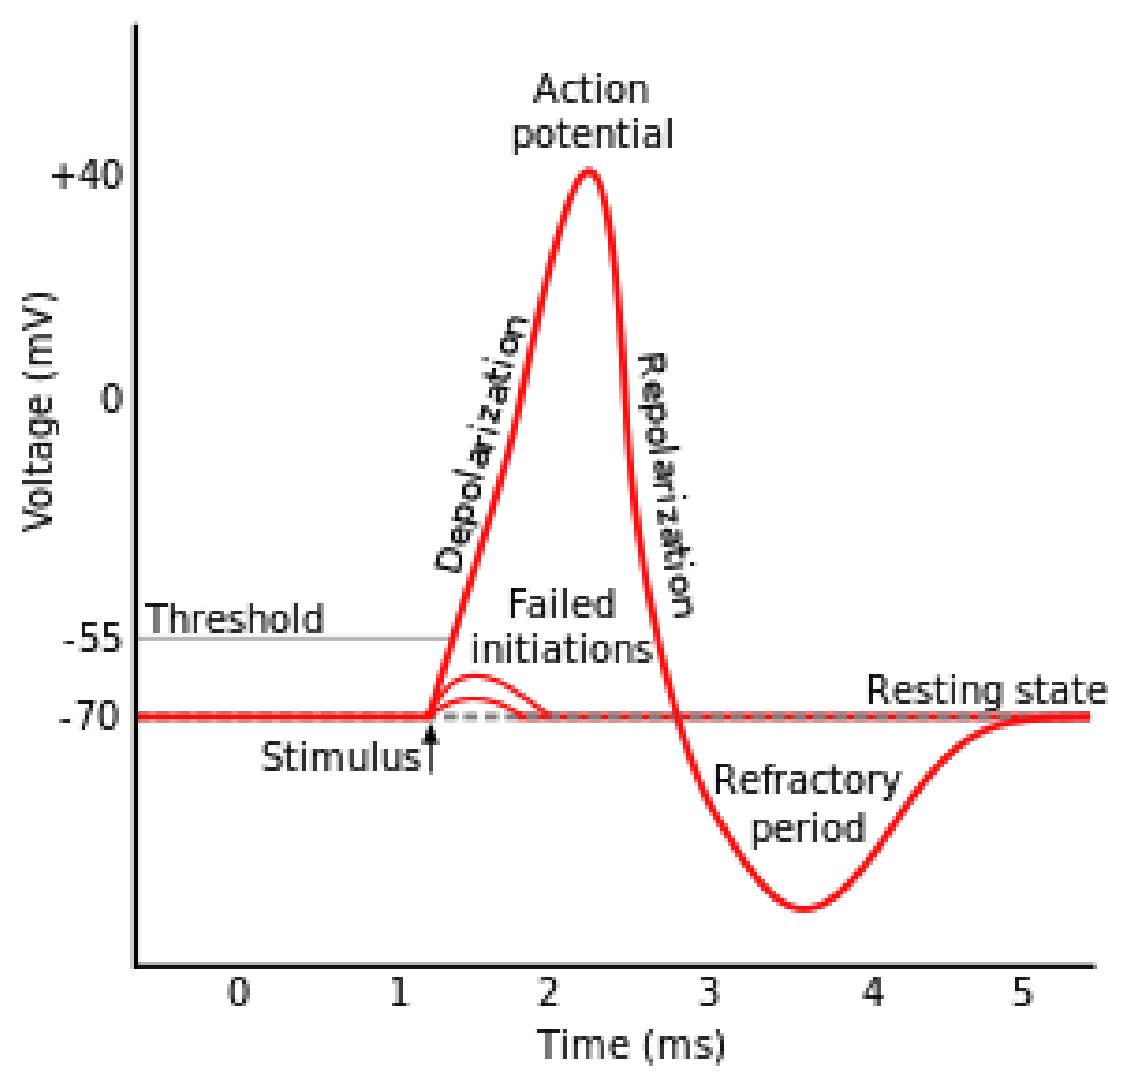
\includegraphics[width=0.4\textwidth]{assets/biological-neuron-activation}
    \caption{~Representation of action potentials and the triggering threshold needed to propagate a signal~\cite{ann-basics}}\label{fig:bio-neuron-activation}
\end{figure}


\section{Neurons}\label{sec:neurons}

Now let's look at a mathematical model of an \textit{artificial neuron}.
This model contains three input nodes: $X_1$, $X_2$, and $X_3$, that channel their output values multiplied by their respective weights $w_{11}$, $w_{12}$, and $w_{13}$, into the neuron ``body.''
We denote $n$ dendrites in the input layer nodes as $x_1$, $x_2$, $x_3$, \ldots, $x_n$ and their corresponding $m$ weights as $w_{11}$, $w_{12}$, \ldots, $w_{nm}$, where $w_{ij}$ refers to the weight taking $x_j$ to the node $i$.
The body of an artificial neuron works simply by summing input values multiplied by the connection \textit{weights} along with the neuron \textit{``bias''} term $b$ (this can be thought of as neuron resting-state potential) and passes the summed value to an $activation function$.
The activation function is usually one of the nonlinear transfer functions described later.
This value is either fed into the following layer of neurons or outputted out of the model.
A simplified model of the artificial neuron can be seen in figure~\ref{fig:artificial-neuron}.~\cite{ann-basics}


\begin{figure}
    \centering
    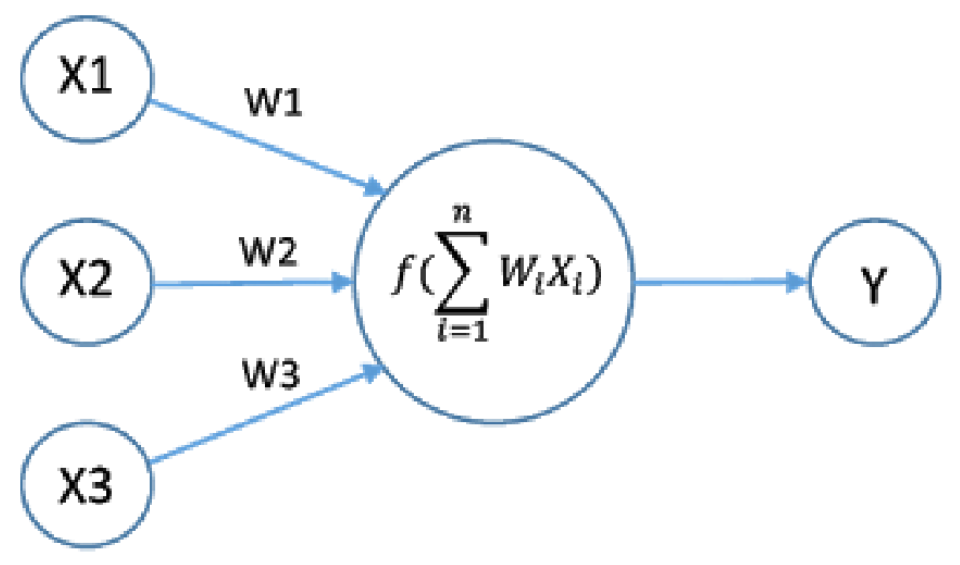
\includegraphics[width=0.4\textwidth]{assets/artificial-neuron}
    \caption{~A mathematical depiction of an artificial neuron~\cite{ann-basics}}\label{fig:artificial-neuron}
\end{figure}

A mathematical formula for neuron internal potential is following: \[ y = (w_{11}, w_{12}, \ldots, w_{1n}) \times
\begin{blockarray}{c}
    \begin{block}{[c]}
        x_{11} \\
        x_{12} \\
        x_{13} \\
        \vdots \\
        x_{1n} \\
    \end{block}%
\end{blockarray}%
= w_{11}x_1 + w_{12}x_2 + \ldots + w_{1n}x_n + b = \textbf{w} \times \textbf{x} + b
\]

Later we apply an \textit{activation function} (figure~\ref{fig:activation-functions}) $\sigma$ to the node’s \textit{internal potential}, $\sigma (y)$ is the output of a single neuron.
The activation function corresponds to the activation state of a node.
As mentioned earlier, a voltage potential must build up enough signal in the cell body to send a signal down the axon.
The activation function simulates this biological effect in a neural network for the node and output signal.
Overall, this is how we model a single neuron.
A \textit{neural network} is a collection of single neurons arranged into layers.
Therefore, by understanding how a single neuron works, we can better grasp how a neural network functions.~\cite{ann-basics}


\section{Activation functions}\label{sec:activation-functions}

The \textit{activation function}, also known as the \textit{transfer function}, corresponds to the activation state of a neuron.
It simulates the biological effect of overcoming a voltage potential to propagate to an axon.
This function manipulates internal potential (pre-state) and transforms it into the output coming from a node.
Mathematically, the transfer function $\sigma (r)$ has to be differentiable (to allow backpropagation), increasing, and has to have horizontal asymptotes.
$r$ corresponds to a pre-state for which the activation function generates an output.
A couple of typical functions for $\sigma (r)$ will be discussed.~\cite{ann-basics}

These are the formulas for the most common functions:

\begin{align*}
    \sigma (r) &= arctan(r) = tan^{-1}(r), \\[4pt]
    \sigma (r) &= sigmoid(r) = \frac{1}{1 + e^{-r}}, \\[4pt]
    \sigma (r) &= \frac{e^{2r} - 1}{e^{2r} + 1}, \\[4pt]
    \sigma (r) &= reLU(r) = max(0, r)
\end{align*}

You can see these four activation functions plotted in a graph in figure~\ref{fig:activation-functions}.

\begin{figure}
    \centering
    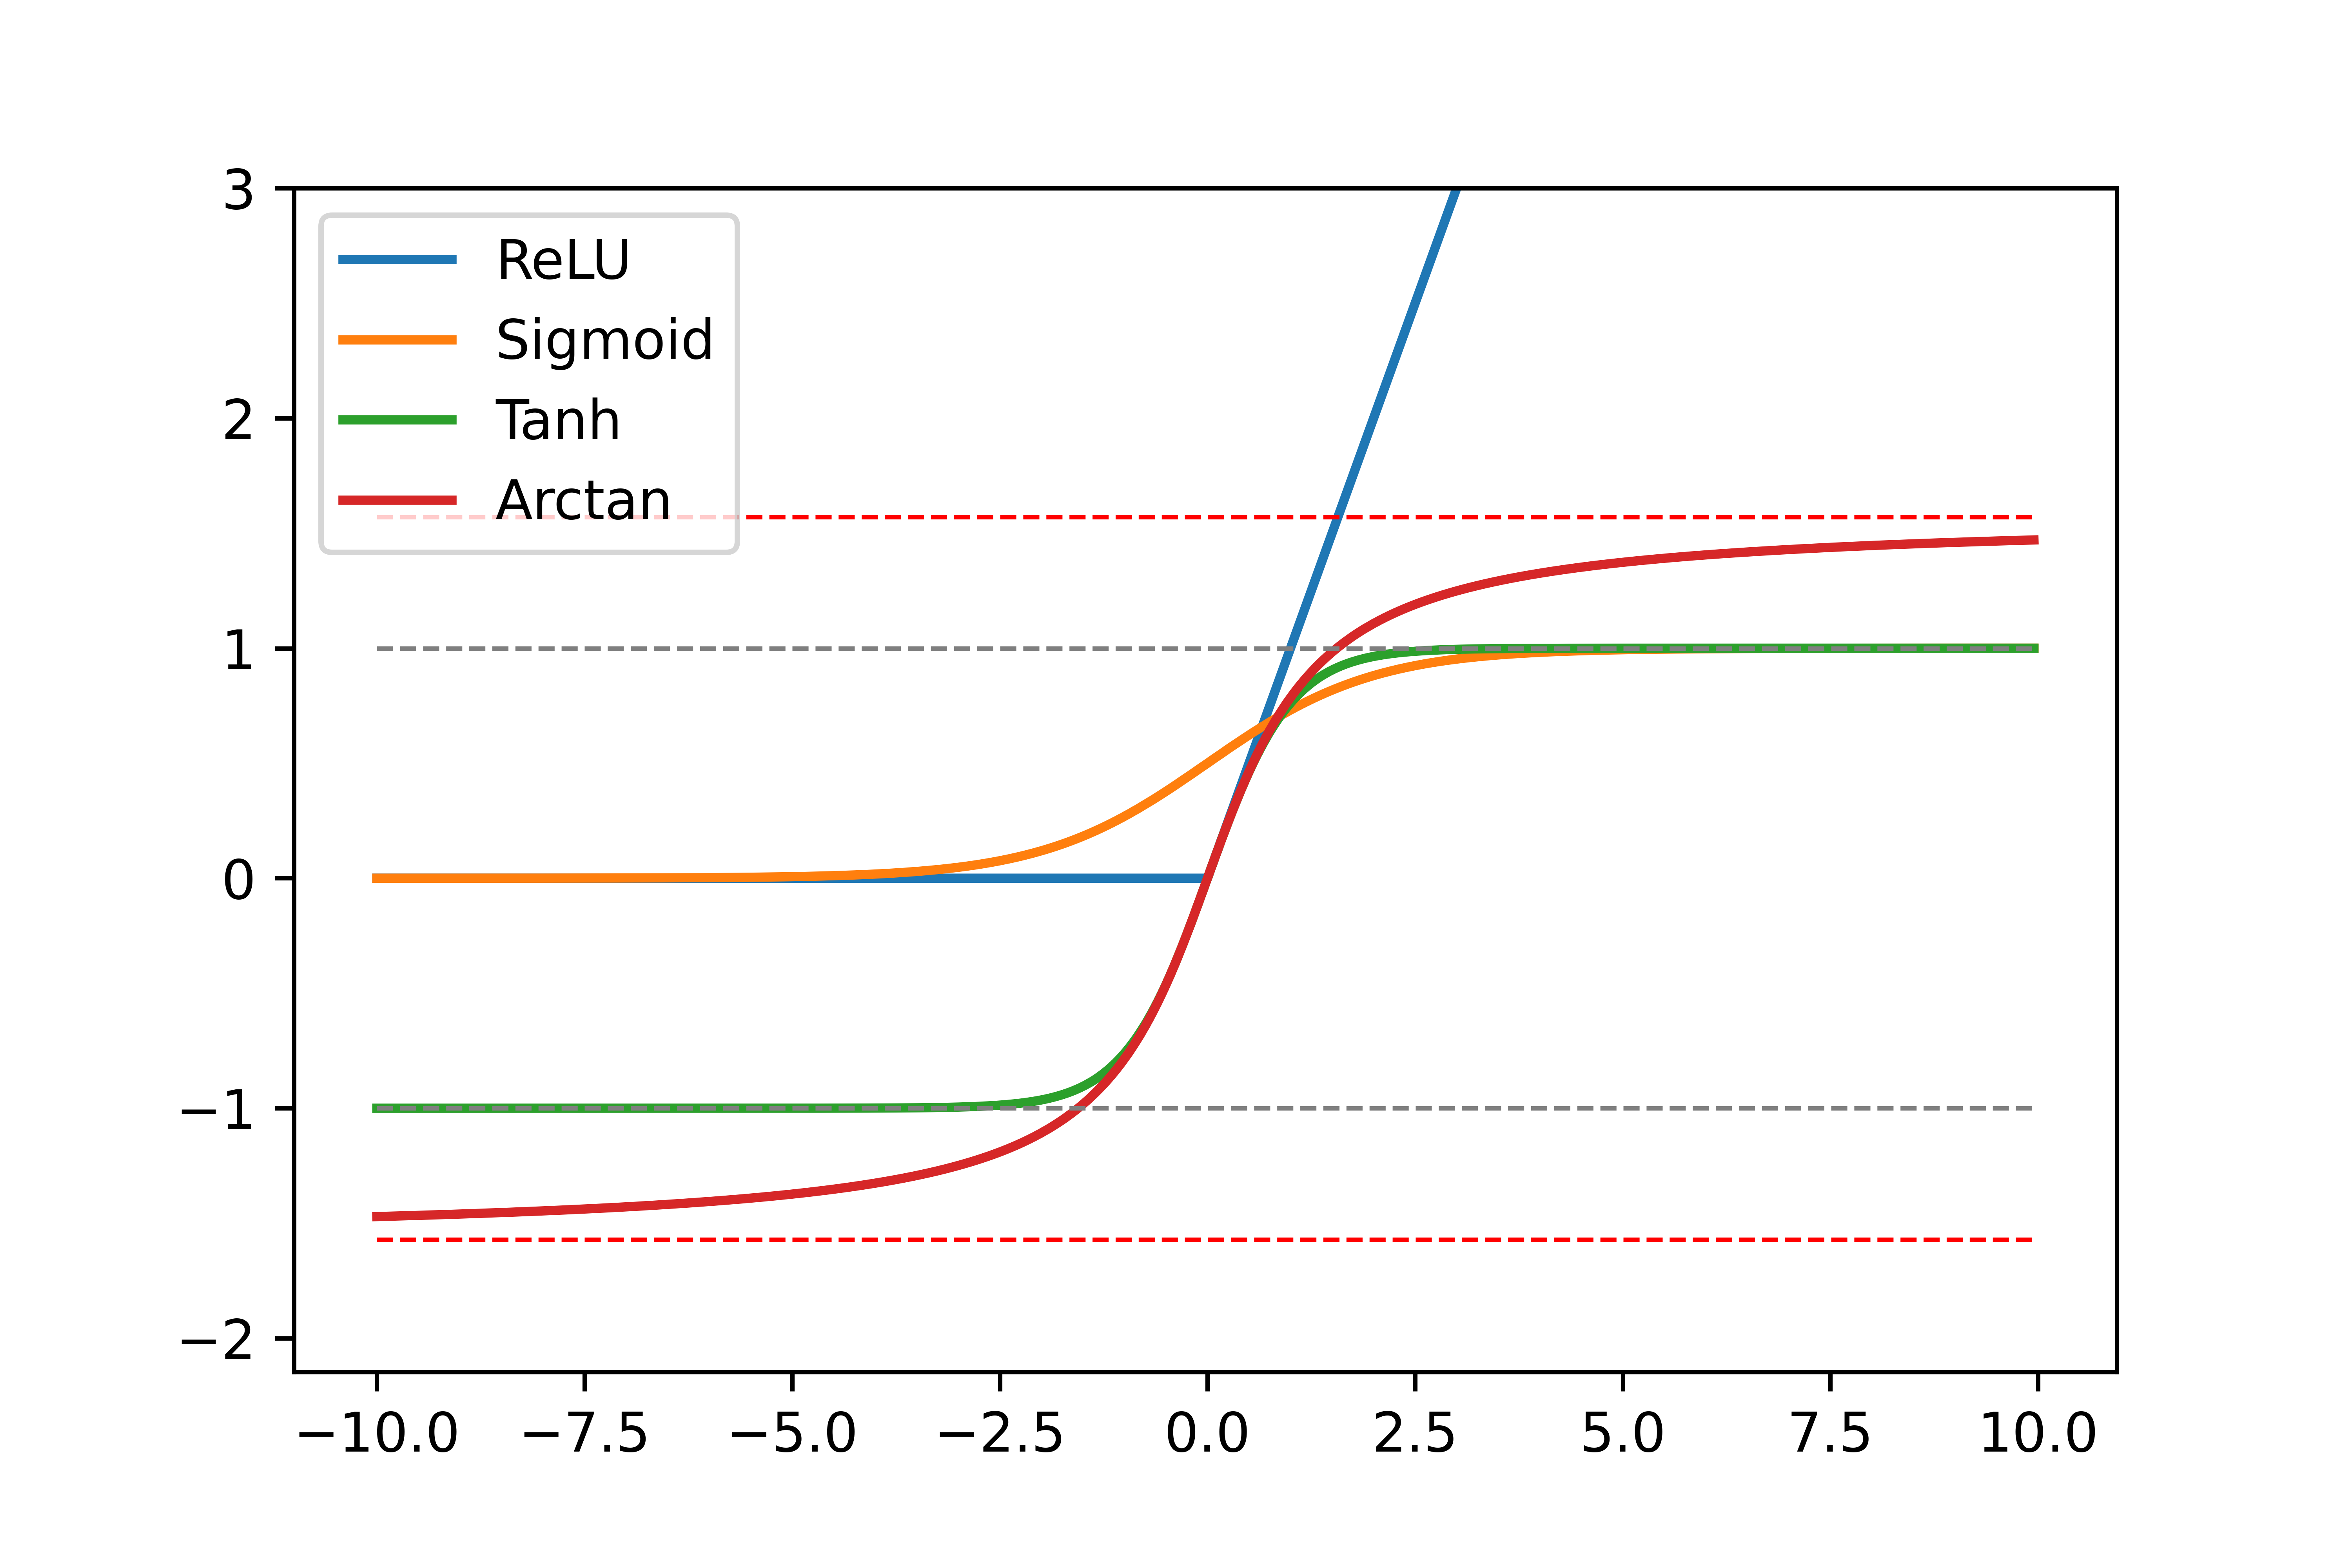
\includegraphics[width=0.7\textwidth]{assets/activation-functions}
    \caption{~Commonly used activation functions}\label{fig:activation-functions}
\end{figure}


\section{Network architecture}\label{sec:network-architecture}

A neural network consists of a sequence of \textit{layers}.
The first layer is called the \textit{input layer}, and the number of neurons (or nodes) in the input layer is derived from the \textit{dimensionality} of the input: $x_i \in \mathbb{R}^n$, the layer has $n$ nodes.
The final layer is called the output layer, and the number of neurons in the output layer is derived from the dimensionality of the output: $y_j \in \mathbb{R}^m$, the layer has $m$ nodes.
In Figure~\ref{fig:ann-architecture}, $x_i \in \mathbb{R}^3$ and $y_j \in \mathbb{R}^1$ so, there are three neurons in the input layer and one neuron in the output layer.
In between the two layers mentioned before are a number of the hidden layers, each containing some number of k neurons.
We define the neural network's \textit{architecture} by the number of nodes in each layer.
For example, figure~\ref{fig:ann-architecture} depicts a neural network with three nodes in the input layer, four nodes in the first hidden layer, four nodes in the second hidden layer, and one node in the output layer.
This network could be described as a 3-4-4-1 neural network.~\cite{ann-basics}


\begin{figure}
    \centering
    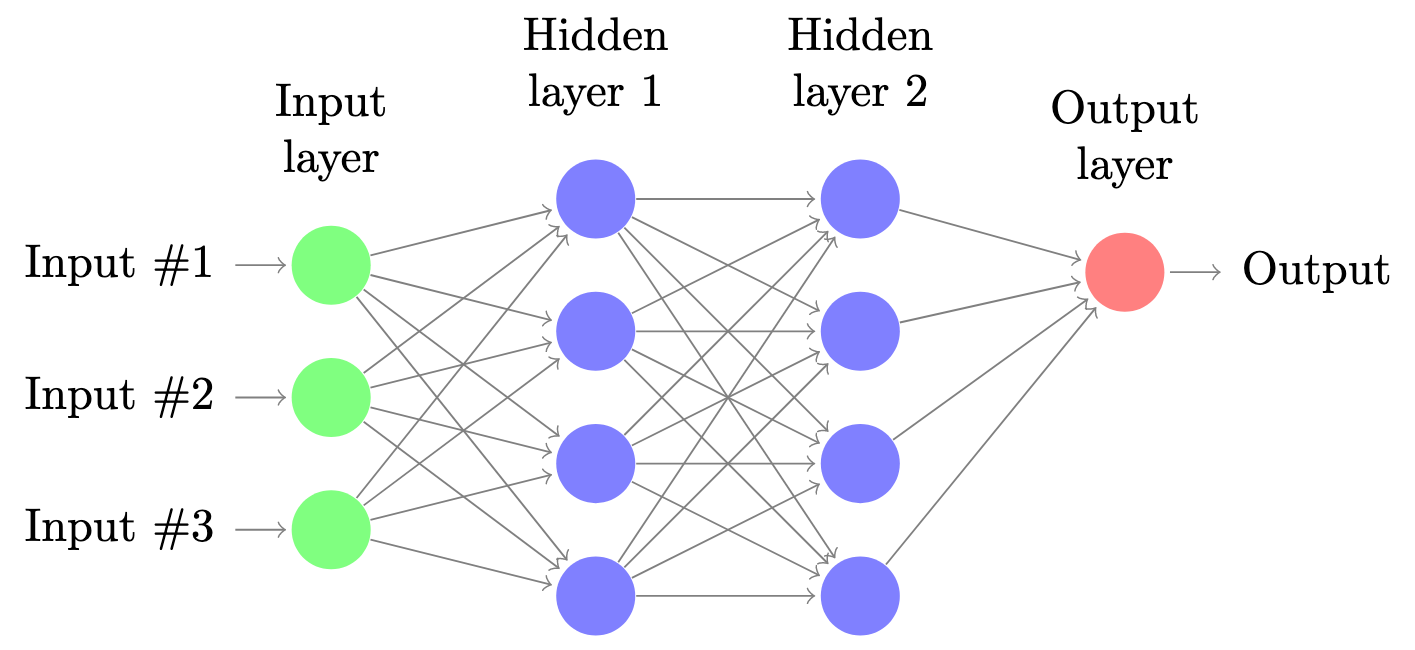
\includegraphics[width=\textwidth]{assets/ann-architecture}
    \caption{~A 3-4-4-1 neural network~\cite{ann-basics}}\label{fig:ann-architecture}
\end{figure}


\section{Training and application of ANNs}\label{sec:training-and-application-of-anns}

A neural network is a model that, when trained, \textit{recognizes patterns} in data sets.
Once a neural net is \textit{trained}, given enough simulation data to recognize the patterns, it can predict outputs in future data.
We can think of training a neural network as \textit{estimating a function} between a given domain and range.
Once trained, any data within the domain we provide can be mapped to the range of the function.
A simple example of a neural network in action is data \textit{classification}.
We are given a data set containing six characteristics of 200 wines (the input would be a $6 \times 200$ matrix) and knowing the properties of 5 different types of wine.
We can train the neural network on 50 different wines, and then the generated function will be able to classify the other 150 wines into the five types of wine (the output would be a $5 \times 200$ matrix).
ANNs can be a powerful tool for \textit{analyzing}, \textit{predicting}, or \textit{generating} data.~\cite{ann-basics}

There are two types of learning: \textit{supervised} learning and \textit{unsupervised} learning.
Supervised learning is when the output or target values are known.
That was the case in the beforementioned example about the wine classification.
In classifying wine into the five types, we knew the correct wine types for the 200 bottles when used as a learning dataset.
Contrary to that, unsupervised learning does not ``know'' the outputs or target values.
The learning process finds \textit{patterns} within the data in order to output values.
Unsupervised learning is used in many complex systems, including data processing, modeling, and classification.
The goal of the training process is to find weight and bias values that produce the most accurate function approximation.
That is easier said than done as there are many caveats when using and training neural networks, like choosing unsuitable network architecture.~\cite{ann-basics}


\section{Feed-Forward Neural Networks}\label{sec:feed-forward-neural-networks}

A \textit{feed-forward} neural network is one of the most straightforward ANN architectures.
It is a part of supervised learning and creates a mapping $\mathbb{R}^n \to \mathbb{R}^m$.
The mapping consists of an initial signal $x$, pre-states $P_j$, activation function $\sigma (r)$, and states $S_j$.
In order to compute the neural network's final output, we have to calculate all these states for each layer.
We start at the input layer and continue forward towards the output layer because each layer depends on the previous one.~\cite{ann-basics}

These are the formulas for calculating pre-states $P_j$ and states $S_j$:

\[
    P_i = W_i S_{i-1} + b_i, S_i = \sigma (P_i)
\]


\section{Backpropagation}\label{sec:backpropagation}

The goal of a neural network is to approximate a function between a given range and domain.
Our aim is to build the function so that the determined outputs equal the given target values, $F (x_i) = \hat y_i$, where $F$ is the function created by ANN, $x_i$ the inputs, and $\hat y_i$ the target values.
The typical to go about this is to create a \textit{loss function} that computes the error between our prediction $\hat y_i$ and the actual output $y_i$.
We then find the values of parameters that minimize it.
The loss function depends on what type of problem we are solving.
\textbf{Mean Squared Error} is mainly used for regression and \textbf{Categorical Cross-Entropy} is most commonly used for classification.~\cite{ann-basics}
Since we know the targets $y_i$ and the outputs $\hat y_i = F (x_i)$ (as we just described earlier), our error functions will be the following:

Mean Squared Error: \[ L=(y_i - \hat y_i)^2 \]

Categorical Cross-Entropy (given M classes): \[ L=\sum_{i=1}^{M} y_i \log \hat y_i \]

The loss function is dependent on the weight matrices $W_i$ and the bias vectors $b_i$ for each layer of the neural network.
In order to decrease the error of the neural net, we will use the \textit{gradient} of the error function.
We calculate the \textit{derivative} of the loss function, compute the \textit{direction of the gradient} and change the weights and biases to move in the \textit{opposite} direction of the gradient.
Moving in the direction of the gradient achieves the fastest ascend, so moving in the direction opposite to the gradient results in the fastest descent.~\cite{ann-basics}
Unsurprisingly this method is called \textit{gradient descent}, where the parameter $u$ (the actual parameters of the function are the weights $W_i$ and biases $b_i$) is updated by:
\[ u_{new} = u_{old} - \alpha \frac{dL}{du} \]

Where α is the learning rate, controlling how big the leaps are taken when updating the weights and biases to reduce error.
\textit{``Generally, a large learning rate allows the model to learn faster, at the cost of arriving on a sub-optimal final set of weights.
A smaller learning rate may allow the model to learn a more optimal or even globally optimal set of weights but may take significantly longer to train.''}~\cite{learning-rate}
We use backpropagation in order to determine the term $\frac{dL}{du}$.
While there are other techniques (like genetic algorithms), \textit{backpropagation} of error is an efficient way of computing the change of the error in a network.
For backpropagation, we first run a  forward pass through the network to determine each node's state conditions.
We determine the partial derivatives through the network to get each node's error term $\Delta^l_m$ when going backward.~\cite{ann-basics}
Following is the formula to update the weight $W^l_{mn}$, which connects node $n$ in layer $l - 1$ to node $m$ in layer $l$:

\[
        \mathit{new}\, W^l_{mn} = W^l_{mn} + \varepsilon \frac{dL}{dW} = W^l_{mn} + \varepsilon \Delta^l_m S^{l-1}_n
\]

$\Delta^l_m$ here means the error term that measures how much node $m$ in layer $l$ was responsible for overall errors in our output, and $S^{l-1}_n$ is the state of node $n$ in layer $l-1$.
$\Delta^l_m$ is defined explicitly as $\delta^L_j = (\hat y_j - y_j ) \sigma '(P^L_j)$ for the output layer $L$ and recursively for preceding layers $l = 1, 2,\, \ldots, L - 1$ as $ \Delta^l_m = \sigma '(P^l_m) \sum_{j \in l+2} \Delta^{l+1}_j W^{l+1}_{jm}$.~\cite{ann-basics}
For updating the biases, following formula is used:

\[
    new \, b^l_k = b^l_k + \varepsilon \frac{dL}{db} = b^l_k + \varepsilon \Delta^l_k
\]


% Transformer architecture
%---------------------------------------------------------------


\chapter{The Transformer architecture}\label{ch:transformer-architecture}

\begin{chapterabstract}
    The Transformer is a unique ANN architecture researched at Google Brain and proposed in 2017 in the paper "Attention Is All You Need\cite{attention-is-all-you-need}."
    The model was a massive success in the natural language processing field.
    It was first designed for machine translation but has since been adapted to many other NLP tasks like text classification, text generation\cite{gpt1, gpt2, gpt3}, text summarization, question answering, and was even extended to work in computer vision\cite{dert, vision-transformer, image-transformer}.
\end{chapterabstract}


\section{Overview}\label{sec:overview}

The Transformer model takes advantage of an \textit{encoder-decoder} structure.
The encoder maps the input sequence $x = (x_1, \ldots, x_n)$ to a sequence of continuous representations $z = (z_1, \ldots, z_n)$.
We then pass representation $z$ to the decoder that generates the final output sequence $y = (y_1, \ldots, y_m)$ one symbol at a time.
At each step, the model is \textit{auto-regressive}, meaning it consumes previously generated symbols as additional input for the following step.
The Transformer implements this architecture using stacked point-wise, fully connected layers and self-attention for both the encoder and the decoder.
Please see the overall structure of the Transformer in figure~\ref{fig:transformer-overview}.~\cite{attention-is-all-you-need}


\begin{figure}
    \centering
    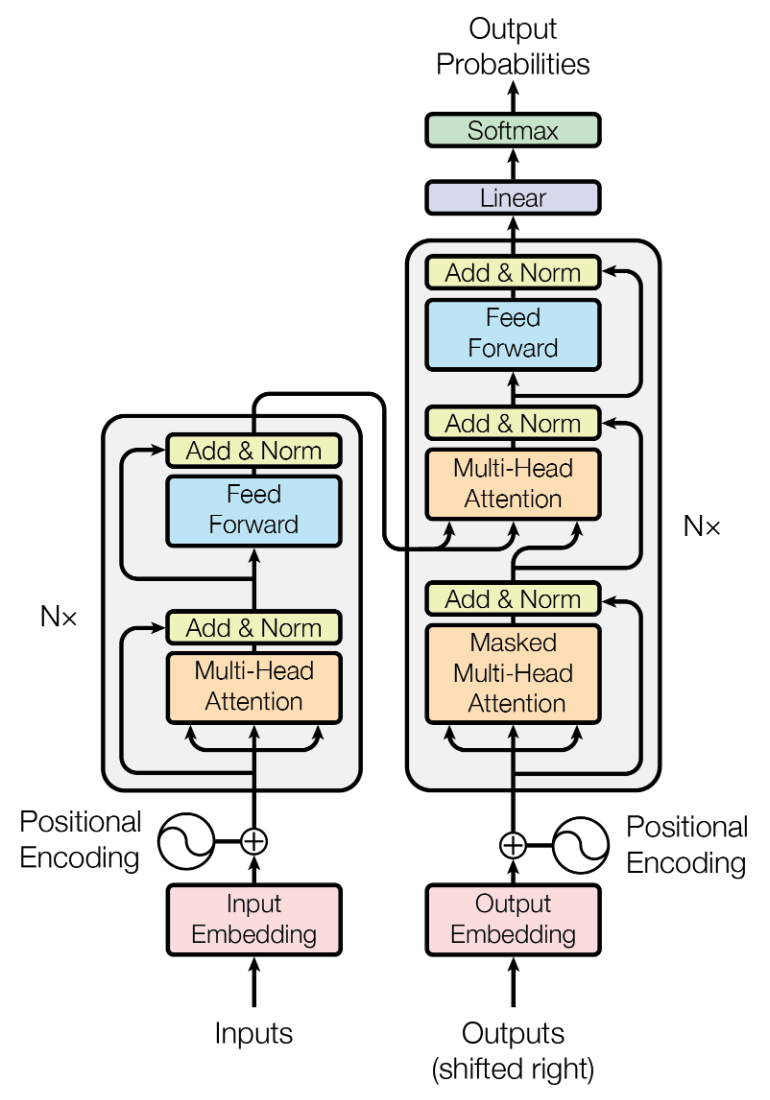
\includegraphics[width=0.6\textwidth]{assets/transformer-overview}
    \caption{~The Transformer - model architecture~\cite{attention-is-all-you-need}}\label{fig:transformer-overview}
\end{figure}


\section{Encoder}\label{sec:encoder}

The \textit{encoder} is formed of a stack of $N = 6$ identical layers.
Each layer has two sub-layers;
a \textit{multi-head self-attention} mechanism and a simple, position-wise, fully connected \textit{feed-forward network}.
The sub-layers use a \textit{residual connection}\footnote{residual connection means that not only consecutive layers are connected, but there are also additional connections bypassing a certain number of layers\cite{residual-connection}} around each of the two sub-layers, followed by layer normalization\cite{layer-normalization}.
To sum it up, the output of each sub-layer is $LayerNorm(x + Sublayer(x))$, where $Sublayer(x)$ is the function implemented by the sub-layer itself (self-attention/feed-forward ANN).
To enable these residual connections, all sub-layers in the model and the embedding layers produce outputs of dimension $d_{\text{model}} = 512$.
Visualization of the encoder module can be seen in figure~\ref{fig:encoder-decoder-detail}.~\cite{attention-is-all-you-need}


\begin{figure}
    \centering
    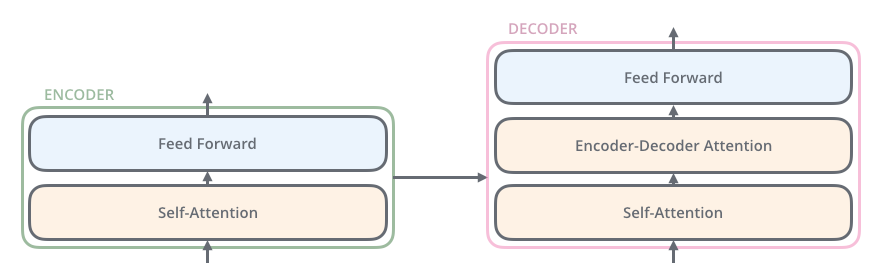
\includegraphics[width=0.86\textwidth]{assets/encoder-decoder-detail}
    \caption{~The encoder and decoder module detail~\cite{illustrated-transformer}}\label{fig:encoder-decoder-detail}
\end{figure}


\section{Decoder}\label{sec:decoder}


The \textit{decoder} comprises a stack of $N = 6$ identical layers as well.
The decoder module uses the same two sub-layers (just like the encoder) but, in addition to that, introduces a third sub-layer, which performs multi-head attention over the encoder's stack output.
Analogous to the encoder, we use layer normalization and residual connections when connecting sub-layers.
The \textit{self-attention} sub-layer in the decoder is modified to forbid positions from attending to successive positions.
Using this masking (also called teacher-forcing) and the fact that the output embeddings are shifted by one position ensures that predictions for an $i^{th}$ position depend exclusively on known positions less than $i$.~\cite{attention-is-all-you-need}
The decoder and its relation to the encoder can be seen in figure~\ref{fig:encoder-decoder-detail}.


\section{Attention}\label{sec:attention}

\textit{Attention} is the heart of the Transformer architecture;
it maps a \textit{query} and a set of \textit{key}-\textit{value} pairs to an output.
The output is computed as a sum weighted by a compatibility function of the query with the corresponding key.
The query, keys, and values are all represented as vectors.~\cite{attention-is-all-you-need}
The representation of attention can be seen in figure~\ref{fig:attention}.


\begin{figure}
    \centering
    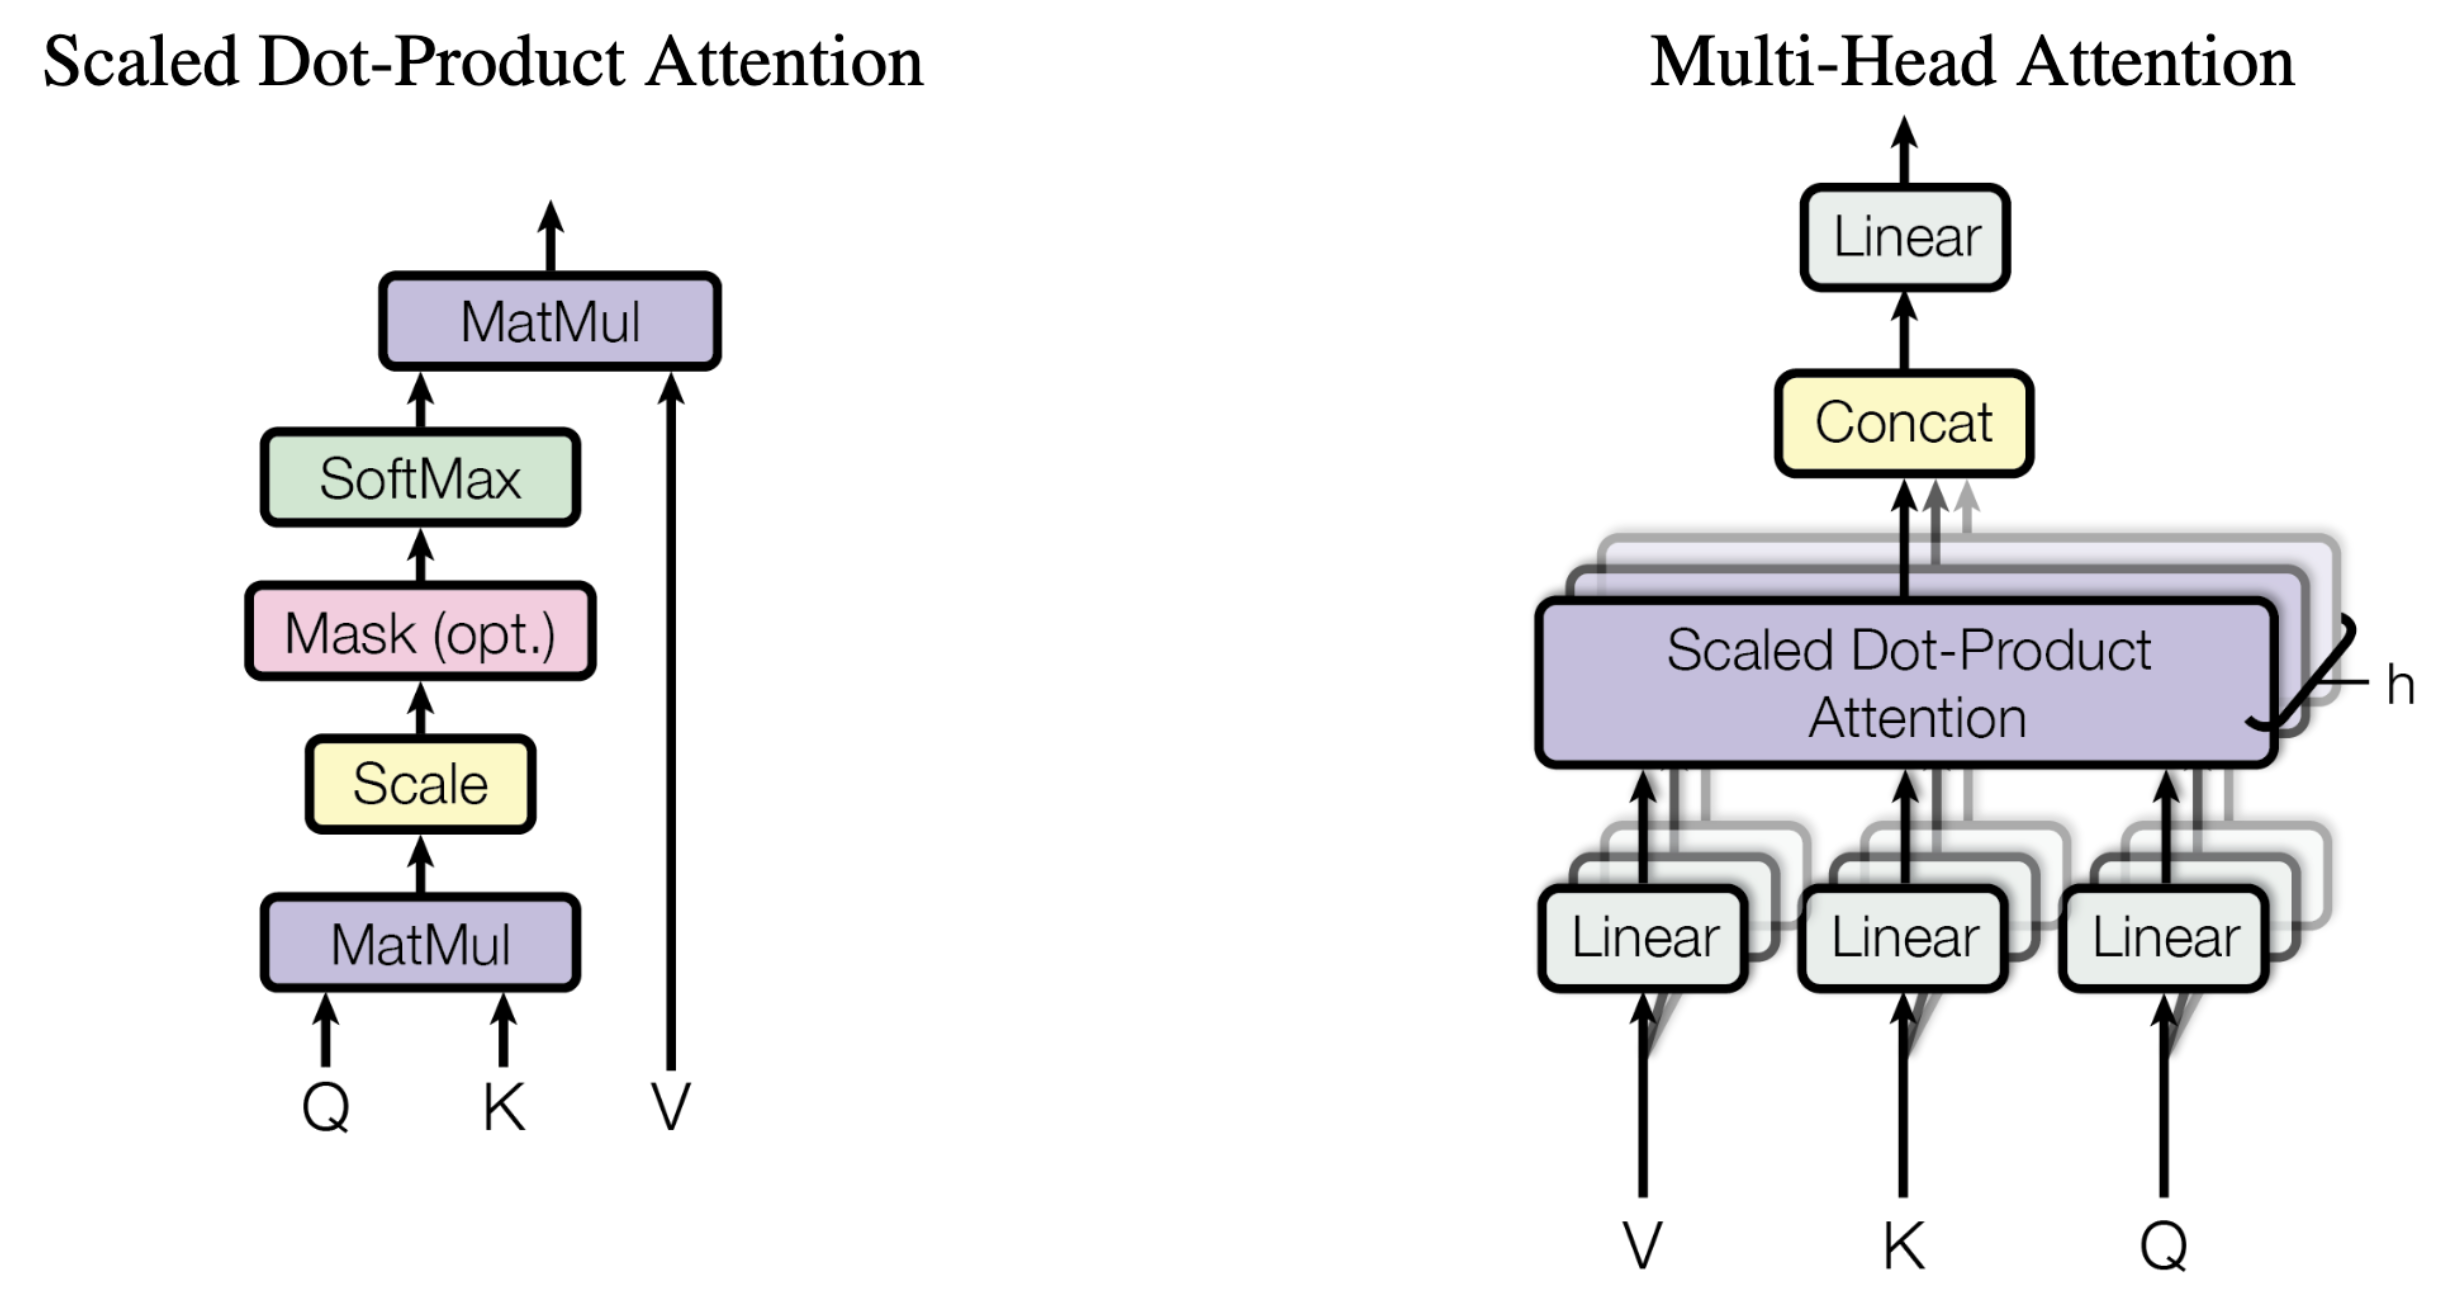
\includegraphics[width=\textwidth]{assets/attention}
    \caption{~Depiction of Scaled-Dot-Product Attention (left) and Multi-Head Attention (right)~\cite{attention-is-all-you-need}}\label{fig:attention}
\end{figure}

\subsection{Scaled Dot-Product Attention}\label{subsec:scaled-dot-product-attention}

The input for "Scaled Dot-Product Attention" consists of \textit{queries}, \textit{keys}, and \textit{values}.
The keys and queries take up dimension $d_k$, and the values take up dimension $d_v$.
The weights of values are computed by calculating the dot products of the query with all keys, each divided by $\sqrt{d_k}$, and finally, a \textit{softmax functio} is applied.
In practice, the attention function is computed on a set of queries, values, and keys simultaneously by packing them into \textit{matrices} \textbf{Q}, \textbf{K}, and \textbf{V}, respectively.~\cite{attention-is-all-you-need}
The matrix of outputs is computed as: \[ Attention(Q, K, V ) = softmax( \frac{QK^T}{\sqrt{d_k}}) V \]

The authors suspect that for large values of $d_k$, the dot products grow large in magnitude, pushing the softmax function into regions with minimal gradients.
Hence, to counteract this effect, the dot products are scaled by $\frac{1}{\sqrt{d_k}}$.~\cite{attention-is-all-you-need}

\subsection{Multi-Head Attention}\label{subsec:multi-head-attention}

The authors found that instead of using \textit{Scaled Dot-Product Attention} isolated, it is beneficial to \textit{linearly project} queries, keys, and values $h$ times with different learned linear projections to $d_k$, $d_k$, and $d_v$ dimensions.
The attention function is computed on all these projected versions of Q, K, and V in parallel, yielding $d_v$-dimensional output values.
Those are then concatenated and projected again, resulting in the final values.
Multi-head attention allows the model to attend to information from different representation subspaces at different positions at once.~\cite{attention-is-all-you-need}
Following is the formula for \textit{Multi-Head Attention}:

\begin{align*}
    MultiHead(Q, K, V) &= Concat(head_1, \ldots, head_h) W^O \\
    \text{where }head_i &= Attention(QW^Q_i, KW^K_i, VW^V_i)
\end{align*}

The projections are parameter matrices $W^Q_i \in \mathbb{R}^{d_{\text{model}} \times d_k}$, $W^K_i \in \mathbb{R}^{d_{\text{model}} \times d_k}$, $W^V_i \in \mathbb{R}^{d_{\text{model}} \times d_v}$, and $W^O \in \mathbb{R}^{hd_v \times d_{\text{model}}}$.


\subsection{Use of Attention inside the Transformer}\label{subsec:use-of-attention-inside-the-transformer}

Multi-head attention is used in three different places inside the Transformer.
The first occurrence is in the \textit{encoder-decoder layers}.
The queries come from the previous decoder layer, and keys and values come as outputs from the decoder.
Another way the multi-head attention is used is \textit{self-attention} (figure~\ref{fig:self-attention})), that is, when queries, keys, and values are all taken from the same place, in this case, from the output of the previous layer in the encoder.
The decoder also contains self-attention layers to allow all positions in the decoder to attend to any of the previous positions.
It must be prevented from attending a position that is after a given position to retain \textit{auto-regressivity}.
This is implemented inside the scaled dot-product attention by masking out all following values in the input.~\cite{attention-is-all-you-need}

\begin{figure}
    \centering
    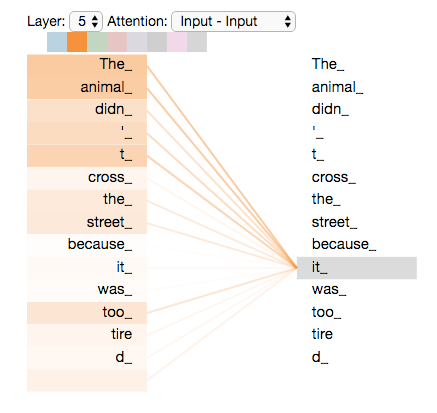
\includegraphics[width=0.5\textwidth]{assets/self-attention}
    \caption{~High-level depiction of self-Attention~\cite{illustrated-transformer}}\label{fig:self-attention}
\end{figure}

\section{Feed-forward networks}\label{sec:feed-forward-networks}

Aside from attention sub-layers, each layer in our encoder and decoder module contains a \textit{fully connected feed-forward} network applied to each position separately and identically~\cite{attention-is-all-you-need}.
The operation composes of two linear transformations with a ReLU activation in between:
\[
    \text{FFN}(x) = max(0, xW1 + b1)W2 + b2
\]
The input and output dimensions are $d_{model} = 512$, and the inner-layer has dimensionality $d_{ff} = 2048$~\cite{attention-is-all-you-need}.

\section{Embeddings and Softmax}\label{sec:embeddings-and-softmax}

The model uses learned \textit{embeddings}\footnote{\textit{``Embeddings are functions that map raw input data to low-dimensional vector representations, while preserving important semantic information about the inputs.''}\cite{embeddings}} to convert the input tokens and output tokens to vectors of the $d_{model}$ dimension.
The \textit{softmax function} converts the decoder output to predicted \textit{next token probabilities}.
The Transformer model shares the same weight matrix between the two embedding layers and the pre-softmax linear transformation.
The weights are then multiplied by $d_{model}$ in the embedding layers.~\cite{attention-is-all-you-need}

\section{Positional encoding}\label{sec:positional-encoding}

The model does not use any \textit{recurrent} or \textit{convolutional} layers, so for the model to understand the positions of all elements, we must provide additional information about the \textit{relative or absolute position} of the tokens in a sequence.
We add \textit{positional encodings} to the input embeddings at the bottoms of the encoder and decoder stacks to provide this information.
The positional encodings have the same dimension $d_{\text{model}}$ as the input embeddings to make summing possible.~\cite{attention-is-all-you-need}
Position encodings in the Transformer are calculated using the following formulas:
\begin{align*}
    PE(pos,2i) &= \sin (pos/10000^{2i/d_{\text{model}}}) \\
    PE(pos,2i+1) &= \cos (pos/10000^{2i/d_{\text{model}}})
\end{align*}
Where $i$ is the dimension and $pos$ is the position.
This results in each dimension of the positional encoding corresponding to a \textit{sinusoid}.
The \textit{wavelengths} create a geometric progression from $2\pi$ to $10000 \cdot 2\pi$.
The authors chose the sinusoidal version as they hypothesize it may allow the model to extrapolate to sequence lengths longer than the ones encountered during training.~\cite{attention-is-all-you-need}





